\documentclass[a4paper, 12pt]{article}

% packages
\usepackage{amssymb}
\usepackage[fleqn]{mathtools}
\usepackage{tikz}
\usepackage{enumerate}
\usepackage{bussproofs}
\usepackage{xcolor}
\usepackage[margin=1.3cm]{geometry}
\usepackage{logicproof}
\usepackage{diagbox}
\usepackage{listings}
\usepackage{graphicx}
\usepackage{lstautogobble}
\usepackage{hyperref}
\usepackage{multirow}
\usepackage{tipa}
\usepackage{pgfplots}
\usepackage{adjustbox}

% tikz libraries
\usetikzlibrary{
    decorations.pathreplacing,
    arrows,
    shapes,
    shapes.gates.logic.US,
    circuits.logic.US,
    calc,
    automata,
    positioning,
    intersections
}

\pgfplotsset{compat=1.16}

\pgfmathdeclarefunction{gauss}{2}{%
  \pgfmathparse{1/(#2*sqrt(2*pi))*exp(-((x-#1)^2)/(2*#2^2))}%
}

\allowdisplaybreaks % allow environments to break
\setlength\parindent{0pt} % no indent

% shorthand for verbatim
% this clashes with logicproof, so maybe fix this at some point?
\catcode`~=\active
\def~#1~{\texttt{#1}}

% code listing
\lstdefinestyle{main}{
    numberstyle=\tiny,
    breaklines=true,
    showspaces=false,
    showstringspaces=false,
    tabsize=2,
    numbers=left,
    basicstyle=\ttfamily,
    columns=fixed,
    fontadjust=true,
    basewidth=0.5em,
    autogobble,
    xleftmargin=3.0ex,
    mathescape=true
}
\newcommand{\dollar}{\mbox{\textdollar}} %
\lstset{style=main}

% augmented matrix
\makeatletter
\renewcommand*\env@matrix[1][*\c@MaxMatrixCols c]{%
\hskip -\arraycolsep
\let\@ifnextchar\new@ifnextchar
\array{#1}}
\makeatother

% ceiling / floor
\DeclarePairedDelimiter{\ceil}{\lceil}{\rceil}
\DeclarePairedDelimiter{\floor}{\lfloor}{\rfloor}

% custom commands
\newcommand{\indefint}[2]{\int #1 \, \mathrm{d}#2}
\newcommand{\defint}[4]{\int_{#1}^{#2} #3 \, \mathrm{d}#4}
\newcommand{\pdif}[2]{\frac{\partial #1}{\partial #2}}
\newcommand{\dif}[2]{\frac{\mathrm{d}#1}{\mathrm{d}#2}}
\newcommand{\limit}[2]{\raisebox{0.5ex}{\scalebox{0.8}{$\displaystyle{\lim_{#1 \to #2}}$}}}
\newcommand{\limitsup}[2]{\raisebox{0.5ex}{\scalebox{0.8}{$\displaystyle{\limsup_{#1 \to #2}}$}}}
\newcommand{\summation}[2]{\sum\limits_{#1}^{#2}}
\newcommand{\product}[2]{\prod\limits_{#1}^{#2}}
\newcommand{\intbracket}[3]{\left[#3\right]_{#1}^{#2}}
\newcommand{\laplace}{\mathcal{L}}
\newcommand{\fourier}{\mathcal{F}}
\newcommand{\mat}[1]{\boldsymbol{#1}}
\renewcommand{\vec}[1]{\boldsymbol{#1}}
\newcommand{\rowt}[1]{\begin{bmatrix}
    #1
\end{bmatrix}^\top}
\DeclareMathOperator*{\argmax}{argmax}
\DeclareMathOperator*{\argmin}{argmin}

\newcommand{\lto}[0]{\leadsto\ }

\newcommand{\ulsmash}[1]{\underline{\smash{#1}}}

\newcommand{\powerset}[0]{\wp}
\renewcommand{\emptyset}[0]{\varnothing}

\makeatletter
\newsavebox{\@brx}
\newcommand{\llangle}[1][]{\savebox{\@brx}{\(\m@th{#1\langle}\)}%
  \mathopen{\copy\@brx\kern-0.5\wd\@brx\usebox{\@brx}}}
\newcommand{\rrangle}[1][]{\savebox{\@brx}{\(\m@th{#1\rangle}\)}%
  \mathclose{\copy\@brx\kern-0.5\wd\@brx\usebox{\@brx}}}
\makeatother
\newcommand{\lla}{\llangle}
\newcommand{\rra}{\rrangle}
\newcommand{\la}{\langle}
\newcommand{\ra}{\rangle}
\newcommand{\crnr}[1]{\text{\textopencorner} #1 \text{\textcorner}}
\newcommand{\bnfsep}[0]{\ |\ }
\newcommand{\concsep}[0]{\ ||\ }

\newcommand{\axiom}[1]{\AxiomC{#1}}
\newcommand{\unary}[1]{\UnaryInfC{#1}}
\newcommand{\binary}[1]{\BinaryInfC{#1}}
\newcommand{\trinary}[1]{\TrinaryInfC{#1}}
\newcommand{\quaternary}[1]{\QuaternaryInfC{#1}}
\newcommand{\quinary}[1]{\QuinaryInfC{#1}}
\newcommand{\dproof}[0]{\DisplayProof}
\newcommand{\llabel}[1]{\LeftLabel{\scriptsize #1}}
\newcommand{\rlabel}[1]{\RightLabel{\scriptsize #1}}

\newcommand{\ttbs}{\char`\\}
\newcommand{\lrbt}[0]{\ \bullet\ }

% colours
\newcommand{\violet}[1]{\textcolor{violet}{#1}}
\newcommand{\blue}[1]{\textcolor{blue}{#1}}
\newcommand{\red}[1]{\textcolor{red}{#1}}
\newcommand{\teal}[1]{\textcolor{teal}{#1}}

% reasoning proofs
\usepackage{ltablex}
\usepackage{environ}
\keepXColumns
\NewEnviron{reasoning}{
    \begin{tabularx}{\textwidth}{rlX}
        \BODY
    \end{tabularx}
}
\newcommand{\proofline}[3]{$(#1)$ & $#2$ & \hfill #3 \smallskip \\}
\newcommand{\proofarbitrary}[1]{& take arbitrary $#1$ \smallskip \\}
\newcommand{\prooftext}[1]{\multicolumn{3}{l}{#1} \smallskip \\}
\newcommand{\proofmath}[3]{$#1$ & = $#2$ & \hfill #3 \smallskip \\}
\newcommand{\prooftherefore}[1]{& $\therefore #1$ \smallskip \\}
\newcommand{\proofbc}[0]{\prooftext{\textbf{Base Case}}}
\newcommand{\proofis}[0]{\prooftext{\textbf{Inductive Step}}}

% ER diagrams
\newcommand{\nattribute}[4]{
    \node[draw, state, inner sep=0cm, minimum size=0.2cm, label=#3:{#4}] (#1) at (#2) {};
}
\newcommand{\mattribute}[4]{
    \node[draw, state, accepting, inner sep=0cm, minimum size=0.2cm, label=#3:{#4}] (#1) at (#2) {};
}
\newcommand{\dattribute}[4]{
    \node[draw, state, dashed, inner sep=0cm, minimum size=0.2cm, label=#3:{#4}] (#1) at (#2) {};
}
\newcommand{\entity}[3]{
    \node[] (#1-c) at (#2) {#3};
    \node[inner sep=0cm] (#1-l) at ($(#1-c) + (-1, 0)$) {};
    \node[inner sep=0cm] (#1-r) at ($(#1-c) + (1, 0)$) {};
    \node[inner sep=0cm] (#1-u) at ($(#1-c) + (0, 0.5)$) {};
    \node[inner sep=0cm] (#1-d) at ($(#1-c) + (0, -0.5)$) {};
    \draw
    ($(#1-c) + (-1, 0.5)$) -- ($(#1-c) + (1, 0.5)$) -- ($(#1-c) + (1, -0.5)$) -- ($(#1-c) + (-1, -0.5)$) -- cycle;
}
\newcommand{\relationship}[3]{
    \node[] (#1-c) at (#2) {#3};
    \node[inner sep=0cm] (#1-l) at ($(#1-c) + (-1, 0)$) {};
    \node[inner sep=0cm] (#1-r) at ($(#1-c) + (1, 0)$) {};
    \node[inner sep=0cm] (#1-u) at ($(#1-c) + (0, 1)$) {};
    \node[inner sep=0cm] (#1-d) at ($(#1-c) + (0, -1)$) {};
    \draw
    ($(#1-c) + (-1, 0)$) -- ($(#1-c) + (0, 1)$) -- ($(#1-c) + (1, 0)$) -- ($(#1-c) + (0, -1)$) -- cycle;
}

% AVL Trees
\newcommand{\avltri}[4]{
    \draw ($(#1)$) -- ($(#1) + #4*(0.5, -1)$) -- ($(#1) + #4*(-0.5, -1)$) -- cycle;
    \node at ($(#1) + #4*(0, -1) + (0, 0.5)$) {#3};
    \node at ($(#1) + #4*(0, -1) + (0, -0.5)$) {#2};
}

% RB Trees
\tikzset{rbtr/.style={inner sep=2pt, circle, draw=black, fill=red}}
\tikzset{rbtb/.style={inner sep=2pt, circle, draw=black, fill=black}}

% Samples
\tikzset{spos/.style={inner sep=2pt, circle, draw=black, fill=blue!20}}
\tikzset{sneg/.style={inner sep=2pt, circle, draw=black, fill=red!20}}

% Joins
\newcommand\ljoin{\stackrel{\mathclap{\normalfont\mbox{\tiny L}}}{\bowtie}}
\newcommand\rjoin{\stackrel{\mathclap{\normalfont\mbox{\tiny R}}}{\bowtie}}
\newcommand\ojoin{\stackrel{\mathclap{\normalfont\mbox{\tiny O}}}{\bowtie}}

\setcounter{MaxMatrixCols}{100}

% actual document
\begin{document}
    {\sc Computing $3^\text{rd}$ Year Notes} \hfill ~https://github.com/lin-e/imperial-revision~
    \rule{\textwidth}{0.1pt}
    \section*{CO395 - Introduction to Machine Learning \hfill (70050)}
        \subsection*{Week 2 (Introduction to ML)}
        \subsection*{Week 3 (Instance-based Learning + Decision Trees)}
            The \textbf{k Nearest Neighbours (k-NN)} classifier is classified as a \textbf{lazy learner}.
            A lazy learner stores all the training examples in the data set, and postpone any processing until a request is made (such as a prediction).
            On the other hand, \textbf{decision trees} are classified as a \textbf{eager learner}.
            An eager learner will attempt to construct a general target decision function, which is prepared prior to a query being made.
            \subsubsection*{Classification with Instance-based Learning}
                The concept behind instance-based learning is that we will use samples in a training data set in order to make inference on a query.
                \medskip

                The \textbf{Nearest Neighbour} classifier is a specific example, where it classifies a test instance to the label of the nearest training instance, where nearest is subject to some distance metric.
                This is a \textbf{non-parametric model}, which means it naturally emerges from the training set.
                Note in the example below, an issue with this is that it can be sensitive to noise, as it would classify the \blue{blue} point to be \red{red}, as it is the closest instance in the training set, even though it's more likely to be black - it is very sensitive to noise, and can \textbf{overfit} to the training data.
                \medskip

                On the other hand, if we consider the \textbf{k Nearest Neighbours}, highlighted by the lines in \violet{violet}, we get the class to be black, as we have 4 against 1.
                Usually, we need $k$ to be odd, to ensure a winner for the decision task.
                \begin{center}
                    \begin{tikzpicture}[x=1.5cm]
                        % using CO202's RBT nodes because I'm lazy
                        \node[rbtr] at (0, 0) {};
                        \node[rbtr] at (-3, -1) {};
                        \node[rbtr] at (-1, -1) {};
                        \node[rbtr] at (-2, -2) {};
                        \node[rbtr] at (-3, -3) {};
                        \node[rbtr] at (-1, -3) {};
                        \node[rbtb] at (-2, -4) {};
                        \node[rbtb] at (0, -4) {};
                        \node[rbtb] at (1, -4) {};
                        \node[rbtb] (nn4) at (2, -3) {};
                        \node[rbtr] (nn0) at (2, -2) {};
                        \node[inner sep=2pt, circle, draw=black, fill=blue] (test) at (1, -2) {};
                        \node[rbtb] (nn1) at (1, -0.5) {};
                        \node[rbtb] (nn2) at (1, -3.5) {};
                        \node[rbtb] (nn3) at (2, -1) {};
                        \node[rbtb] at (3, -1) {};
                        \node[rbtb] at (3, -2) {};
                        \node[rbtb] at (4, -2) {};
                        \node[rbtb] at (5, 0) {};

                        \draw
                        (test) edge[dashed] (nn0)
                        (test) edge[dashed, violet] (nn1)
                        (test) edge[dashed, violet] (nn2)
                        (test) edge[dashed, violet] (nn3)
                        (test) edge[dashed, violet] (nn4);
                    \end{tikzpicture}
                \end{center}
                Increasing $k$ will give the classifier have a smoother decision boundary (higher bias), and less sensitive to training data (lower variance).
                Choosing $k$ is dependant on the dataset, normally with a validation dataset.
                \medskip

                The distance metric can be defined in many different ways, including the $\ell_1$, $\ell_2$ and $\ell_\infty$-norms as seen in \textbf{CO233}.
                Other metrics exist such as the \textbf{Mahalanobis distance} for non-isotropic spaces, typically used for Gaussian distributions, or the \textbf{Hamming distance} for binary strings.
                \medskip

                Another variation is the \textbf{Distance Weighted k-NN}.
                For example, we may not want to trust neighbours which are further away, such as in the example below.
                \begin{center}
                    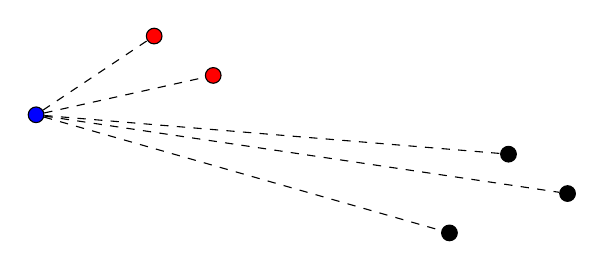
\begin{tikzpicture}[x=1.5cm]
                        \node[inner sep=2pt, circle, draw=black, fill=blue] (test) at (0, 0) {};
                        \node[rbtr] (nn0) at (1, 1) {};
                        \node[rbtr] (nn1) at (1.5, 0.5) {};
                        \node[rbtb] (nn2) at (4, -0.5) {};
                        \node[rbtb] (nn3) at (3.5, -1.5) {};
                        \node[rbtb] (nn4) at (4.5, -1) {};

                        \draw
                        (test) edge[dashed] (nn0)
                        (test) edge[dashed] (nn1)
                        (test) edge[dashed] (nn2)
                        (test) edge[dashed] (nn3)
                        (test) edge[dashed] (nn4);
                    \end{tikzpicture}
                    \hfill
                    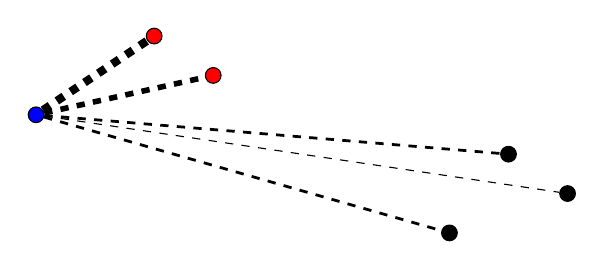
\begin{tikzpicture}[x=1.5cm]
                        \node[inner sep=2pt, circle, draw=black, fill=blue] (test) at (0, 0) {};
                        \node[rbtr] (nn0) at (1, 1) {};
                        \node[rbtr] (nn1) at (1.5, 0.5) {};
                        \node[rbtb] (nn2) at (4, -0.5) {};
                        \node[rbtb] (nn3) at (3.5, -1.5) {};
                        \node[rbtb] (nn4) at (4.5, -1) {};

                        \draw
                        (test) edge[dashed, line width=3pt] (nn0)
                        (test) edge[dashed, line width=2pt] (nn1)
                        (test) edge[dashed, line width=1pt] (nn2)
                        (test) edge[dashed, line width=1pt] (nn3)
                        (test) edge[dashed] (nn4);
                    \end{tikzpicture}
                \end{center}
                The idea is that we add weights to each neighbour (depending on distance), typically a higher weight for closer neighbours.
                We then assign the class based on which class has the largest sum.
                This metric, $w^{(i)}$, is any measure favouring the votes of nearby neighbours, such as;
                \begin{itemize}
                    \itemsep0em
                    \item inverse of distance
                        \[w^{(i)} = \frac{1}{d(x^{(i)}, x^{(q)})}\]
                    \item Gaussian distribution
                        \[w^{(i)} = \frac{1}{\sqrt{2 \pi}}e^{-\frac{d\left(x^{(i)}, x^{(q)}\right)^2}{2}}\]
                \end{itemize}
                The value of $k$ is less important in the weighted case, as distant examples won't greatly affect classification.
                If $k = N$, where $N$ is the size of the training set, it is a global method, otherwise it is a local method (only considering the samples close by).
                This method is also more robust to noisy training data, however it can be slow for large datasets.
                \medskip

                As this method relies on distance metrics, it may not work well if using all features in high dimensional spaces.
                If these features are irrelevant, instances in the same class may be far from each other.
                One solution to this is to weight features differently.
                \medskip

                k-NN can also be used for regression, either by computing the mean value across $k$ nearest neighbours (which leads to a very rough curve), or by using locally weighted regression, which computes the weighted mean value across $k$ nearest neighbours, leading to a smoother curve.
            \subsubsection*{Classification with Decision Trees}
                Decisions trees are the principal of focusing on a subset or single feature of each sample and then make a decision whether it's true or false (for each feature), and repeat this process to finer decisions until we manage to classify the sample that we want to check.
                \medskip

                In decision trees, we learn a succession of linear decision boundaries that we can use to eventually correctly classify samples.
                \begin{center}
                    \hfill
                    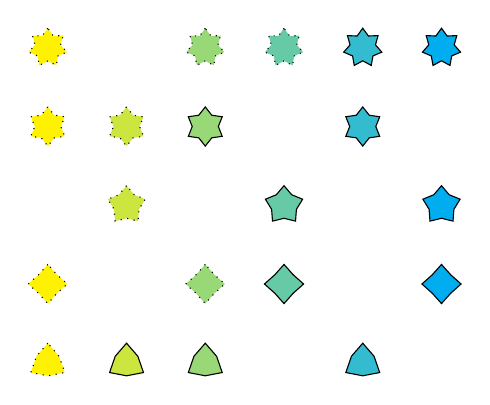
\begin{tikzpicture}
                        \node[dotted, draw, star, star points=3, fill=yellow!100!cyan] at (0, 0) {};
                        \node[dotted, draw, star, star points=4, fill=yellow!100!cyan] at (0, 1) {};
                        \node[dotted, draw, star, star points=6, fill=yellow!100!cyan] at (0, 3) {};
                        \node[dotted, draw, star, star points=7, fill=yellow!100!cyan] at (0, 4) {};

                        \node[draw, star, star points=3, fill=yellow!80!cyan] at (1, 0) {};
                        \node[dotted, draw, star, star points=5, fill=yellow!80!cyan] at (1, 2) {};
                        \node[dotted, draw, star, star points=6, fill=yellow!80!cyan] at (1, 3) {};

                        \node[draw, star, star points=3, fill=yellow!60!cyan] at (2, 0) {};
                        \node[dotted, draw, star, star points=4, fill=yellow!60!cyan] at (2, 1) {};
                        \node[draw, star, star points=6, fill=yellow!60!cyan] at (2, 3) {};
                        \node[dotted, draw, star, star points=7, fill=yellow!60!cyan] at (2, 4) {};

                        \node[draw, star, star points=4, fill=yellow!40!cyan] at (3, 1) {};
                        \node[draw, star, star points=5, fill=yellow!40!cyan] at (3, 2) {};
                        \node[dotted, draw, star, star points=7, fill=yellow!40!cyan] at (3, 4) {};

                        \node[draw, star, star points=3, fill=yellow!20!cyan] at (4, 0) {};
                        \node[draw, star, star points=6, fill=yellow!20!cyan] at (4, 3) {};
                        \node[draw, star, star points=7, fill=yellow!20!cyan] at (4, 4) {};

                        \node[draw, star, star points=4, fill=yellow!0!cyan] at (5, 1) {};
                        \node[draw, star, star points=5, fill=yellow!0!cyan] at (5, 2) {};
                        \node[draw, star, star points=7, fill=yellow!0!cyan] at (5, 4) {};
                    \end{tikzpicture}
                    \hfill
                    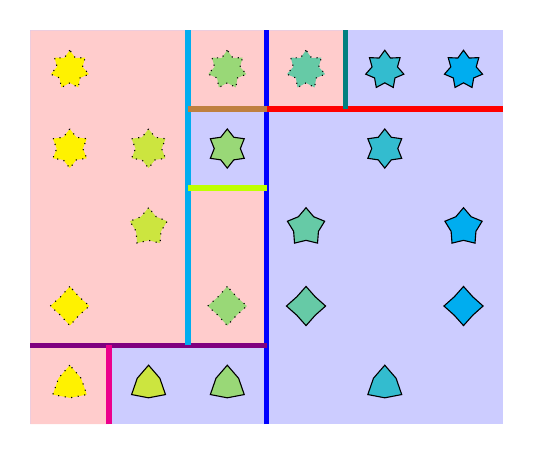
\begin{tikzpicture}
                        \fill[blue!20]
                        (-0.5, -0.5) -- (-0.5, 4.5) -- (5.5, 4.5) -- (5.5, -0.5) -- cycle;
                        \fill[red!20]
                        (-0.5, -0.5) -- (-0.5, 4.5) -- (3.5, 4.5) -- (3.5, 3.5) -- (1.5, 3.5) -- (1.5, 2.5) --(2.5, 2.5) -- (2.5, 0.5) -- (0.5, 0.5) -- (0.5, -0.5) -- cycle;
                        \node[dotted, draw, star, star points=3, fill=yellow!100!cyan] at (0, 0) {};
                        \node[dotted, draw, star, star points=4, fill=yellow!100!cyan] at (0, 1) {};
                        \node[dotted, draw, star, star points=6, fill=yellow!100!cyan] at (0, 3) {};
                        \node[dotted, draw, star, star points=7, fill=yellow!100!cyan] at (0, 4) {};

                        \node[draw, star, star points=3, fill=yellow!80!cyan] at (1, 0) {};
                        \node[dotted, draw, star, star points=5, fill=yellow!80!cyan] at (1, 2) {};
                        \node[dotted, draw, star, star points=6, fill=yellow!80!cyan] at (1, 3) {};

                        \node[draw, star, star points=3, fill=yellow!60!cyan] at (2, 0) {};
                        \node[dotted, draw, star, star points=4, fill=yellow!60!cyan] at (2, 1) {};
                        \node[draw, star, star points=6, fill=yellow!60!cyan] at (2, 3) {};
                        \node[dotted, draw, star, star points=7, fill=yellow!60!cyan] at (2, 4) {};

                        \node[draw, star, star points=4, fill=yellow!40!cyan] at (3, 1) {};
                        \node[draw, star, star points=5, fill=yellow!40!cyan] at (3, 2) {};
                        \node[dotted, draw, star, star points=7, fill=yellow!40!cyan] at (3, 4) {};

                        \node[draw, star, star points=3, fill=yellow!20!cyan] at (4, 0) {};
                        \node[draw, star, star points=6, fill=yellow!20!cyan] at (4, 3) {};
                        \node[draw, star, star points=7, fill=yellow!20!cyan] at (4, 4) {};

                        \node[draw, star, star points=4, fill=yellow!0!cyan] at (5, 1) {};
                        \node[draw, star, star points=5, fill=yellow!0!cyan] at (5, 2) {};
                        \node[draw, star, star points=7, fill=yellow!0!cyan] at (5, 4) {};

                        \draw[blue, line width=2pt] (2.5, -0.5) -- (2.5, 4.5);
                        \draw[red, line width=2pt] (2.5, 3.5) -- (5.5, 3.5);
                        \draw[violet, line width=2pt] (-0.5, 0.5) -- (2.5, 0.5);
                        \draw[teal, line width=2pt] (3.5, 3.5) -- (3.5, 4.5);
                        \draw[magenta, line width=2pt] (0.5, -0.5) -- (0.5, 0.5);
                        \draw[cyan, line width=2pt] (1.5, 0.5) -- (1.5, 4.5);
                        \draw[lime, line width=2pt] (1.5, 2.5) -- (2.5, 2.5);
                        \draw[brown, line width=2pt] (1.5, 3.5) -- (2.5, 3.5);
                    \end{tikzpicture}
                    \hfill
                    \phantom{}
                \end{center}
                In the example above, we repeatedly choose divisions that result in the fewest number of errors, until we are able to classify everything.
                This results in the following decision tree, when we are using the attributes of colour and number of points.
                For brevity, the left branch is the ~false~ branch, ~p~ means points, and ~c~ means colour.
                \begin{center}
                    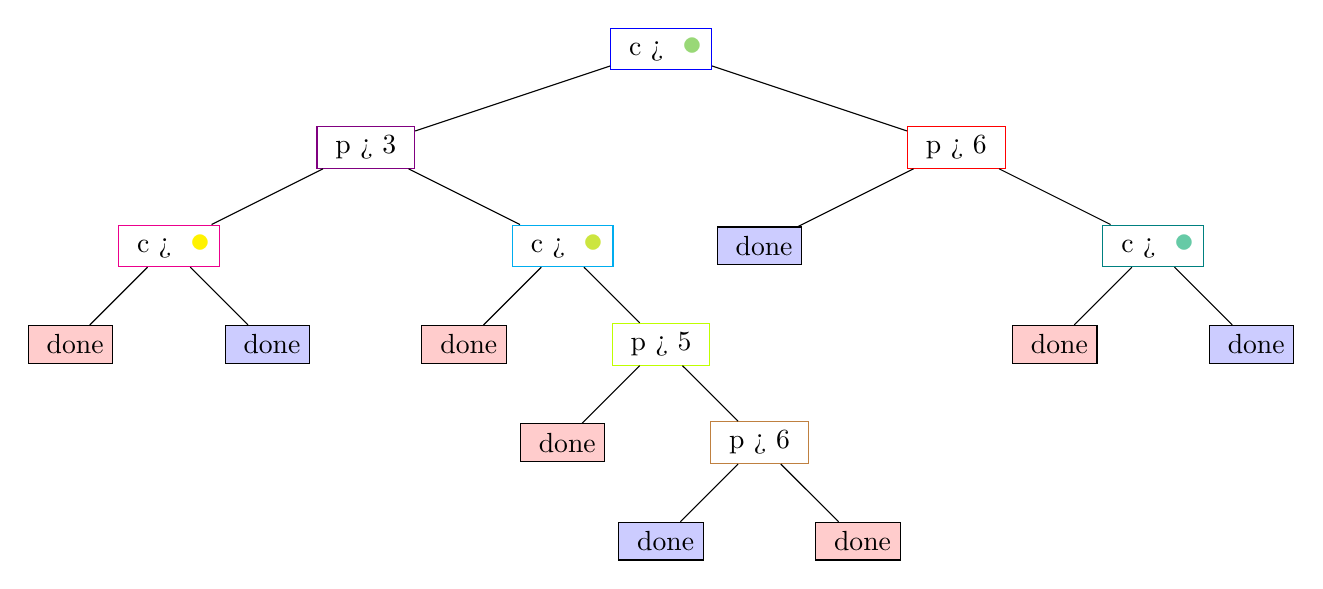
\begin{tikzpicture}[x=1.25cm, y=1.25cm]
                        \node[draw, blue] (o) at (0, 0) {\textcolor{black}{~c > ~}\textcolor{yellow!60!cyan}{\Large$\bullet$}};
                        \node[draw, violet] (ol) at (-3, -1) {\textcolor{black}{~p > 3~}};
                        \node[draw, magenta] (oll) at (-5, -2) {\textcolor{black}{~c > ~}\textcolor{yellow!100!cyan}{\Large$\bullet$}};
                        \node[draw, fill=red!20] (olll) at (-6, -3) {~done~};
                        \node[draw, fill=blue!20] (ollr) at (-4, -3) {~done~};
                        \node[draw, cyan] (olr) at (-1, -2) {\textcolor{black}{~c > ~}\textcolor{yellow!80!cyan}{\Large$\bullet$}};
                        \node[draw, fill=red!20] (olrl) at (-2, -3) {~done~};
                        \node[draw, lime] (olrr) at (0, -3) {\textcolor{black}{~p > 5~}};
                        \node[draw, fill=red!20] (olrrl) at (-1, -4) {~done~};
                        \node[draw, brown] (olrrr) at (1, -4) {\textcolor{black}{~p > 6~}};
                        \node[draw, fill=blue!20] (olrrrl) at (0, -5) {~done~};
                        \node[draw, fill=red!20] (olrrrr) at (2, -5) {~done~};
                        \node[draw, red] (or) at (3, -1) {\textcolor{black}{~p > 6~}};
                        \node[draw, fill=blue!20] (orl) at (1, -2) {~done~};
                        \node[draw, teal] (orr) at (5, -2) {\textcolor{black}{~c > ~}\textcolor{yellow!40!cyan}{\Large$\bullet$}};
                        \node[draw, fill=red!20] (orrl) at (4, -3) {~done~};
                        \node[draw, fill=blue!20] (orrr) at (6, -3) {~done~};

                        \draw
                        (o) -- (ol)
                        (o) -- (or)
                        (ol) -- (oll)
                        (ol) -- (olr)
                        (or) -- (orl)
                        (or) -- (orr)
                        (oll) -- (olll)
                        (oll) -- (ollr)
                        (olr) -- (olrl)
                        (olr) -- (olrr)
                        (orr) -- (orrl)
                        (orr) -- (orrr)
                        (olrr) -- (olrrl)
                        (olrr) -- (olrrr)
                        (olrrr) -- (olrrrl)
                        (olrrr) -- (olrrrr);
                    \end{tikzpicture}
                \end{center}
                Decision trees are a method of approximating discrete classification functions, by representing them as a tree (a set of if-then rules).
                The general algorithm (ID3) for constructing a decision tree is as follows;
                \begin{enumerate}[1.]
                    \itemsep0em
                    \item search for the optimal splitting rule on training data
                    \item split data according to rule
                    \item repeat 1 and 2 on each subset until each subset is pure (only containing a single class)
                \end{enumerate}
            \subsubsection*{How to select the `optimal' split rule}
                Intuitively, we want to partition the datasets such that they are more pure than the original set.
                To do this, we have several metrics;
                \begin{itemize}
                    \itemsep0em
                    \item \textbf{Information gain} \hfill ID3, C4.5
                        \subitem quantifies the reduction of \textbf{entropy}
                    \item \textbf{Gini impurity} \hfill CART
                        \subitem if we randomly select a point in the feature space and randomly classify it according to the class label distribution, what is our probability of getting it incorrect?
                    \item \textbf{Variance reduction} \hfill CART
                        \subitem mostly used for regression trees, with a continuous target variable
                \end{itemize}
                To do this, we need to understand information entropy.
                Entropy is a measure of uncertainty of a random variable.
                It can also be seen as the average amount of information needed to define a random state / variable.
                If something has low entropy, it's predictable, and vice versa for high entropy.
                \medskip

                Imagine we have two boxes, with something stored in one of the two, with an equal probability in each.
                To be fully certain, we need a single bit of information, if it's in the left box, the bit is ~0~, otherwise (if it's in the right box), it's ~1~.
                Similarly, if we have four boxes, with a uniform distribution, we would need 4 bits to encode the 4 states.
                In general;
                \begin{align*}
                    2^B & = K \text{ states} \\
                    B & = \log_2(K) \\
                    I(x) & = \log_2(K) & \text{amount of information to determine the state of a random variable} \\
                    P(x) & = \frac{1}{K} & \Rightarrow \\
                    K & = \frac{1}{K} & \Rightarrow \\
                    I(x) & = -\log_2(P(x))
                \end{align*}
                As such, we can say;
                $$I(x = \text{box}_1) = I(x = \text{box}_2) = I(x = \text{box}_3) = I(x = \text{box}_4) = -\log_2(P(x)) = 2 \text{ bits}$$
                However, assume a non-uniform distribution, with the probabilities being 97\%, 1\%, 1\%, and 1\% respectively.
                If we were told it was in box 1, we do not get a lot of new information (low entropy); however if we were told it was in one of the other three, we high entropy (represents very important information).
                \begin{align*}
                    I(x = \text{box}_1) & = -\log_2(0.97) \\
                    & \approx 0.0439 \text{ bits} \\
                    I(x = \text{box}_2) & = -\log_2(0.1) \\
                    & \approx 6.6439 \text{ bits}
                \end{align*}
                Entropy is defined as the average amount of information;
                $$H(X) = -\summation{k}{K}P(x_k)\log_2(P(x_k))$$
                In our example, we therefore have;
                $$H(X) = -(0.97 \cdot \log_2(0.97) + 0.01 \cdot \log_2(0.01) + 0.01 \cdot \log_2(0.01) + 0.01 \cdot \log_2(0.01)) \approx 0.2419 \text{ bits}$$
                We therefore need, on average, less information to know where the key is (compared to the uniform distribution).
                \medskip

                For continuous entropy, we can use the probability density function $f(x)$ - this is imperfect (it can have negative values), but is still often used in Deep Learning.;
                $$H(X) = - \defint{x}{}{f(x)\log_2(f(x))}{x}$$
                Consider the following example;
                \begin{center}
                    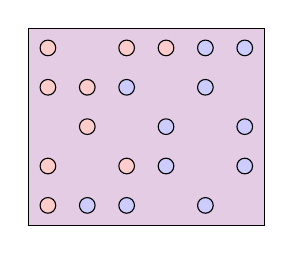
\begin{tikzpicture}[x=0.5cm, y=0.5cm]
                        \draw[fill=violet!20] (-0.5, -0.5) -- (-0.5, 4.5) -- (5.5, 4.5) -- (5.5, -0.5) -- cycle;

                        \node[sneg] at (0, 0) {};
                        \node[sneg] at (0, 1) {};
                        \node[sneg] at (0, 3) {};
                        \node[sneg] at (0, 4) {};

                        \node[spos] at (1, 0) {};
                        \node[sneg] at (1, 2) {};
                        \node[sneg] at (1, 3) {};

                        \node[spos] at (2, 0) {};
                        \node[sneg] at (2, 1) {};
                        \node[spos] at (2, 3) {};
                        \node[sneg] at (2, 4) {};

                        \node[spos] at (3, 1) {};
                        \node[spos] at (3, 2) {};
                        \node[sneg] at (3, 4) {};

                        \node[spos] at (4, 0) {};
                        \node[spos] at (4, 3) {};
                        \node[spos] at (4, 4) {};

                        \node[spos] at (5, 1) {};
                        \node[spos] at (5, 2) {};
                        \node[spos] at (5, 4) {};
                    \end{tikzpicture}
                    \begin{align*}
                        P(\textcolor{blue!20}{\bullet}) & = \frac{11}{20} \\
                        P(\textcolor{red!20}{\bullet}) & = \frac{9}{20} \\
                        H(\textcolor{violet!20}{\blacksquare}) & = -\left(\frac{11}{20} \cdot \log_2\left(\frac{11}{20}\right) + \frac{9}{20} \cdot \log_2\left(\frac{9}{20}\right)\right) \\
                        & \approx 0.9928
                    \end{align*}
                \end{center}
                An entropy value close to 1 would indicate a maximum amount of information needed.
                \begin{center}
                    \hfill
                    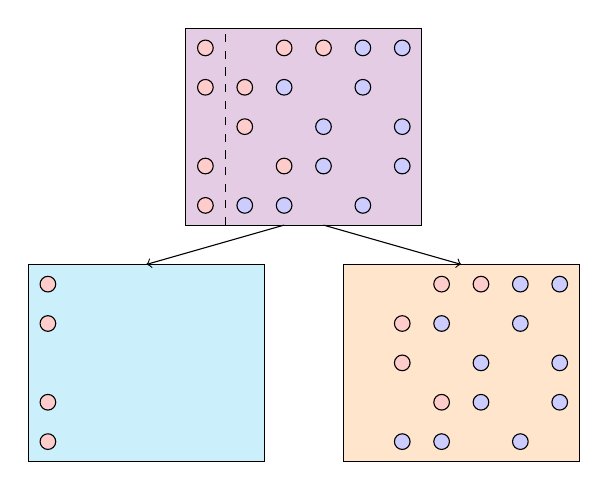
\begin{tikzpicture}[x=0.5cm, y=0.5cm]
                        \begin{scope}[shift={(0, 0)}]
                            \draw[fill=violet!20] (-0.5, -0.5) -- (-0.5, 4.5) -- (5.5, 4.5) -- (5.5, -0.5) -- cycle;

                            \node[sneg] at (0, 0) {};
                            \node[sneg] at (0, 1) {};
                            \node[sneg] at (0, 3) {};
                            \node[sneg] at (0, 4) {};

                            \node[spos] at (1, 0) {};
                            \node[sneg] at (1, 2) {};
                            \node[sneg] at (1, 3) {};

                            \node[spos] at (2, 0) {};
                            \node[sneg] at (2, 1) {};
                            \node[spos] at (2, 3) {};
                            \node[sneg] at (2, 4) {};

                            \node[spos] at (3, 1) {};
                            \node[spos] at (3, 2) {};
                            \node[sneg] at (3, 4) {};

                            \node[spos] at (4, 0) {};
                            \node[spos] at (4, 3) {};
                            \node[spos] at (4, 4) {};

                            \node[spos] at (5, 1) {};
                            \node[spos] at (5, 2) {};
                            \node[spos] at (5, 4) {};

                            \draw (0.5, -0.5) edge[dashed] (0.5, 4.5);
                        \end{scope}
                        \begin{scope}[shift={(-4, -6)}]
                            \draw (-0.5, -0.5)[fill=cyan!20] -- (-0.5, 4.5) -- (5.5, 4.5) -- (5.5, -0.5) -- cycle;

                            \node[sneg] at (0, 0) {};
                            \node[sneg] at (0, 1) {};
                            \node[sneg] at (0, 3) {};
                            \node[sneg] at (0, 4) {};
                        \end{scope}
                        \begin{scope}[shift={(4, -6)}]
                            \draw (-0.5, -0.5)[fill=orange!20] -- (-0.5, 4.5) -- (5.5, 4.5) -- (5.5, -0.5) -- cycle;
                            \node[spos] at (1, 0) {};
                            \node[sneg] at (1, 2) {};
                            \node[sneg] at (1, 3) {};

                            \node[spos] at (2, 0) {};
                            \node[sneg] at (2, 1) {};
                            \node[spos] at (2, 3) {};
                            \node[sneg] at (2, 4) {};

                            \node[spos] at (3, 1) {};
                            \node[spos] at (3, 2) {};
                            \node[sneg] at (3, 4) {};

                            \node[spos] at (4, 0) {};
                            \node[spos] at (4, 3) {};
                            \node[spos] at (4, 4) {};

                            \node[spos] at (5, 1) {};
                            \node[spos] at (5, 2) {};
                            \node[spos] at (5, 4) {};
                        \end{scope}

                        \draw
                        (2, -0.5) edge[->] (-1.5, -1.5)
                        (3, -0.5) edge[->] (6.5, -1.5);
                    \end{tikzpicture}
                    \hfill
                    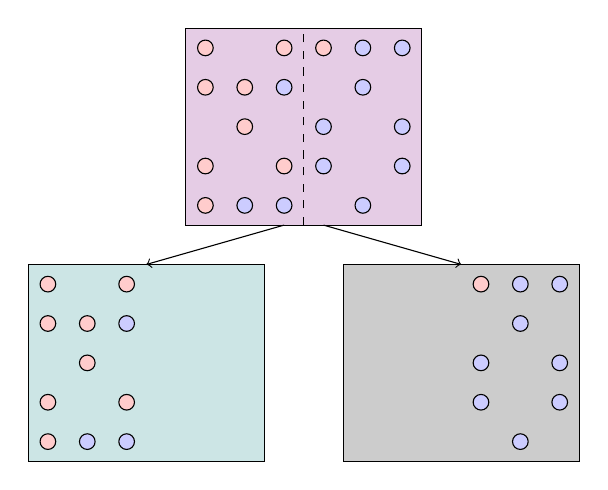
\begin{tikzpicture}[x=0.5cm, y=0.5cm]
                        \begin{scope}[shift={(0, 0)}]
                            \draw[fill=violet!20] (-0.5, -0.5) -- (-0.5, 4.5) -- (5.5, 4.5) -- (5.5, -0.5) -- cycle;

                            \node[sneg] at (0, 0) {};
                            \node[sneg] at (0, 1) {};
                            \node[sneg] at (0, 3) {};
                            \node[sneg] at (0, 4) {};

                            \node[spos] at (1, 0) {};
                            \node[sneg] at (1, 2) {};
                            \node[sneg] at (1, 3) {};

                            \node[spos] at (2, 0) {};
                            \node[sneg] at (2, 1) {};
                            \node[spos] at (2, 3) {};
                            \node[sneg] at (2, 4) {};

                            \node[spos] at (3, 1) {};
                            \node[spos] at (3, 2) {};
                            \node[sneg] at (3, 4) {};

                            \node[spos] at (4, 0) {};
                            \node[spos] at (4, 3) {};
                            \node[spos] at (4, 4) {};

                            \node[spos] at (5, 1) {};
                            \node[spos] at (5, 2) {};
                            \node[spos] at (5, 4) {};

                            \draw (2.5, -0.5) edge[dashed] (2.5, 4.5);
                        \end{scope}
                        \begin{scope}[shift={(-4, -6)}]
                            \draw[fill=teal!20] (-0.5, -0.5) -- (-0.5, 4.5) -- (5.5, 4.5) -- (5.5, -0.5) -- cycle;

                            \node[sneg] at (0, 0) {};
                            \node[sneg] at (0, 1) {};
                            \node[sneg] at (0, 3) {};
                            \node[sneg] at (0, 4) {};

                            \node[spos] at (1, 0) {};
                            \node[sneg] at (1, 2) {};
                            \node[sneg] at (1, 3) {};

                            \node[spos] at (2, 0) {};
                            \node[sneg] at (2, 1) {};
                            \node[spos] at (2, 3) {};
                            \node[sneg] at (2, 4) {};
                        \end{scope}
                        \begin{scope}[shift={(4, -6)}]
                            \draw[fill=black!20] (-0.5, -0.5) -- (-0.5, 4.5) -- (5.5, 4.5) -- (5.5, -0.5) -- cycle;

                            \node[spos] at (3, 1) {};
                            \node[spos] at (3, 2) {};
                            \node[sneg] at (3, 4) {};

                            \node[spos] at (4, 0) {};
                            \node[spos] at (4, 3) {};
                            \node[spos] at (4, 4) {};

                            \node[spos] at (5, 1) {};
                            \node[spos] at (5, 2) {};
                            \node[spos] at (5, 4) {};
                        \end{scope}

                        \draw
                        (2, -0.5) edge[->] (-1.5, -1.5)
                        (3, -0.5) edge[->] (6.5, -1.5);
                    \end{tikzpicture}
                    \hfill
                    \phantom{}
                \end{center}
                \begin{align*}
                    H(\textcolor{cyan!20}{\blacksquare}) & = 0 \\
                    H(\textcolor{orange!20}{\blacksquare}) & \approx 0.896 \\
                    H(\{\textcolor{cyan!20}{\blacksquare}, \textcolor{orange!20}{\blacksquare}\}) & \approx \frac{4}{20} \cdot 0 + \frac{16}{20} \cdot 0.896 \\
                    & \approx 0.7168 \\
                    H(\textcolor{violet!20}{\blacksquare}) - H(\{\textcolor{cyan!20}{\blacksquare}, \textcolor{orange!20}{\blacksquare}\}) & \approx 0.276 & \text{information gain} \\ \\
                    H(\textcolor{teal!20}{\blacksquare}) & \approx 0.8454 \\
                    H(\textcolor{black!20}{\blacksquare}) & \approx 0.5033 \\
                    H(\{\textcolor{teal!20}{\blacksquare}, \textcolor{black!20}{\blacksquare}\}) & \approx \frac{11}{20} \cdot 0.8454 + \frac{9}{20} \cdot 0.5033 \\
                    & \approx 0.6915 \\
                    H(\textcolor{violet!20}{\blacksquare}) - H(\{\textcolor{teal!20}{\blacksquare}, \textcolor{black!20}{\blacksquare}\}) & \approx 0.3013 & \text{information gain} \\ \\
                \end{align*}
                As the second split has the larger information gain, that is the one we will end up selecting (and generally we want to split to maximise information gain).
                A formulation of this is as follows;
                \begin{align*}
                    IG(\text{dataset}, \text{subsets}) & = H(\text{dataset}) - \summation{S \in \text{subsets}}{} \frac{|\ S\ |}{|\ \text{dataset}\ |} H(S) \\
                    |\ \text{dataset}\ | & = \summation{S \in \text{subsets}}{} |\ S\ |
                \end{align*}
                We can have the following types of input;
                \begin{itemize}
                    \itemsep0em
                    \item \textbf{ordered values}
                        \begin{itemize}
                            \itemsep0em
                            \item attribute and split point
                            \item for each attribute, sort the values and consider split points between two examples with different classes
                        \end{itemize}
                    \item \textbf{categorical / symbolic values}
                        \begin{itemize}
                            \itemsep0em
                            \item search for the most informative feature and create as many branches as there are values for this feature
                        \end{itemize}
                \end{itemize}
            \subsubsection*{Worked example for construction decision tree}
                Skipped, as this is basically done for the coursework.
            \subsubsection*{Summary and other considerations with decision tree}
                Note that in general, if we have real-valued attributes, we will end up with a binary tree, with an attribute and threshold at each node.
                On the other hand, if we have categorical values, we can end up with a \textbf{multiway tree}.
                \medskip

                Decision trees will \textbf{overfit}, like with many machine learning algorithms.
                This means the algorithm will take into account every sample in the dataset, to the point where it picks up the noise in the dataset.
                On the other hand, we have an underfitted algorithm, which has low variance and high bias (in contrast).
                \medskip

                In decision trees, to deal with overfitting, we can employ the following strategies;
                \begin{itemize}
                    \itemsep0em
                    \item \textbf{early stopping}
                        \subitem basically stop the algorithm when a condition is met, rather than when the subset is pure (such as maximum depth of tree, or a minimum number of examples in the subset)
                    \item \textbf{pruning} \hfill will be covered more next week
                        \begin{enumerate}[1.]
                            \itemsep0em
                            \item identify internal nodes connected to only leaf nodes
                            \item turn each into a leaf node (with the majority class label)
                            \item if the validation accuracy of the pruned tree is greater, we keep it, and then repeat the process until no other pruning can improve the accuracy
                        \end{enumerate}
                \end{itemize}
                To test this, we can reserve part of the dataset for training, and another part for validation.
                This is called \textbf{cross-validation}.
                \medskip

                Another approach is to use a random forest.
                This involves training multiple decision trees, each with a subset of the training dataset, with a random subset of the features, and therefore each focuses on one subset of the features.
                We then take the majority vote by each of the decision trees as the final outcome.
                \medskip

                Decision trees can also be used for regression (\textbf{regression trees}).
                Instead of class labels, each leaf node predicts a real-valued number.
        \subsection*{Week 4 (Machine Learning Evaluation)}
            \subsubsection*{Evaluation Set-up}
                The goal is to create models and algorithms that can generalise to unseen data.
                We have good accuracy for the training set, since we trained the model for that, however we care more about the accuracy of unknown data.
                \medskip

                To ensure meaningful evaluation, we need to split the training dataset from the test dataset (the test dataset should \textbf{never} be used to train, as it needs to simulate unknown data).
                This is done by first shuffling the dataset, and then splitting it into training and test datasets.
                The training dataset is used to train the model, and the test dataset is then fed into the trained model for final evaluation.
                \medskip

                \textbf{Hyperparameters} are model parameters chosen before the training, such as the $k$ value for $k$-NN algorithm.
                Our overall objective is to find the values that lead to best performance for unknown data.
                An incorrect approach for hyperparameter tuning is to try different values on the training dataset, and then select the ones that lead to the best accuracy on the test dataset.
                This is incorrect because we now use the test dataset as part of the training process, and therefore we cannot say that it is unknown.
                \medskip

                As such, the correct approach is to split the dataset into 3; training, validation, and test.
                The splits for this are between somewhere between $60:20:20$ and $80:10:10$.
                Different hyperparameter values are attempted on the \textbf{training} set, and then the result with the best accuracy on the \textbf{validation} set is chosen.
                The final evaluation is still done on the \textbf{test} dataset.
                \medskip

                We want to keep the classifier that leads to the maximum performance on the validation test.
                We can extend this even further by adding the validation dataset to the training dataset and training it on the model with the best parameters to give it more data.
                Once again, the final evaluation is still done with the test dataset.
                \begin{center}
                    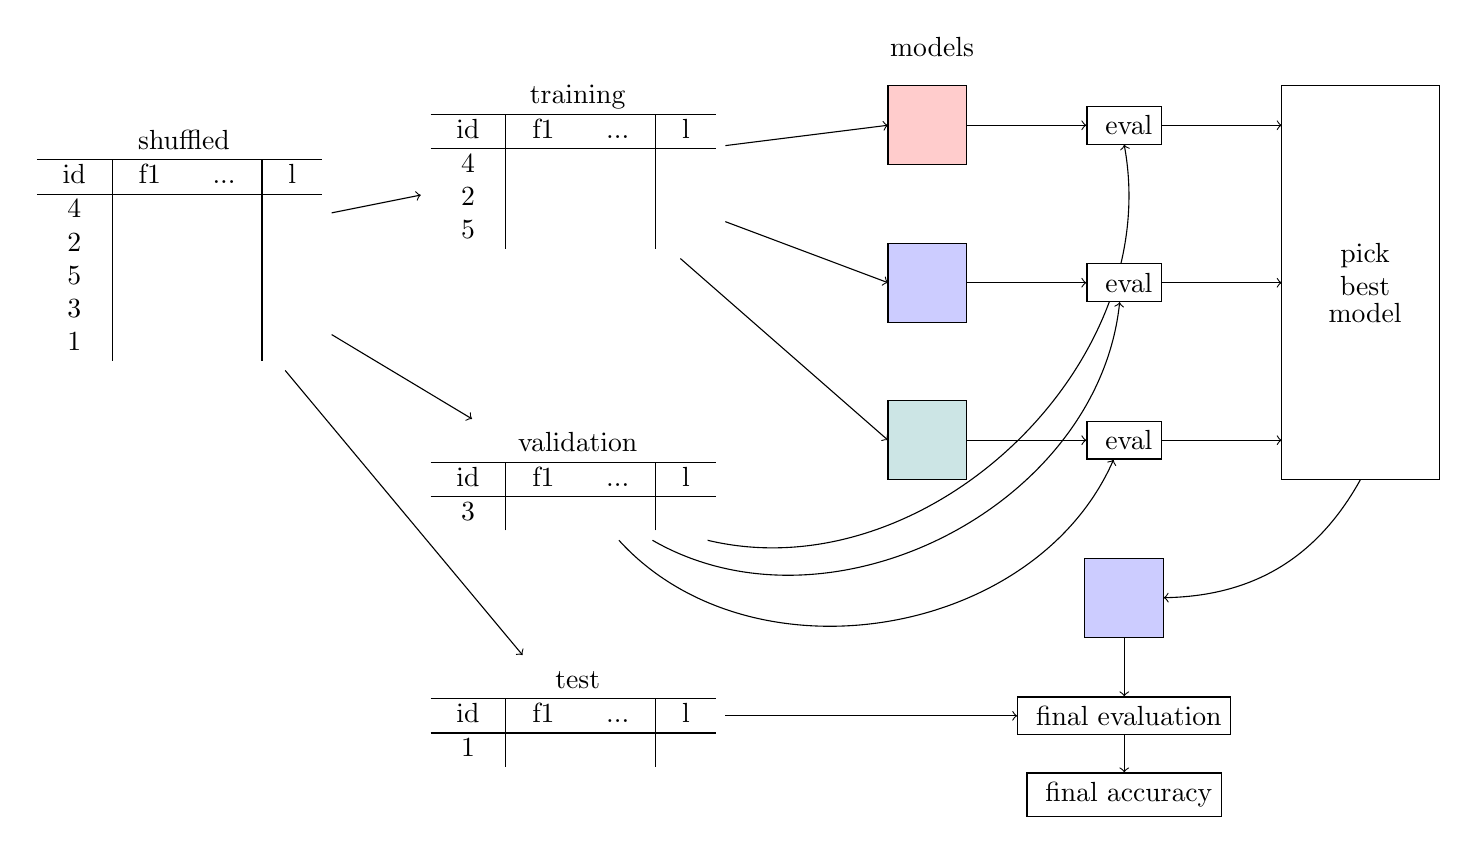
\begin{tikzpicture}
                        \node (shuffled) at (0, 0) {
                            \begin{tabular}{c|cc|c}
                                \multicolumn{4}{c}{~shuffled~} \\
                                \hline
                                ~id~ & ~f1~ & ~...~ & ~l~ \\
                                \hline
                                4 & & & \\
                                2 & & & \\
                                5 & & & \\
                                3 & & & \\
                                1 & & & \\
                            \end{tabular}
                        };
                        \node (training) at (5, 1) {
                            \begin{tabular}{c|cc|c}
                                \multicolumn{4}{c}{~training~} \\
                                \hline
                                ~id~ & ~f1~ & ~...~ & ~l~ \\
                                \hline
                                4 & & & \\
                                2 & & & \\
                                5 & & &
                            \end{tabular}
                        };
                        \node (validation) at (5, -3) {
                            \begin{tabular}{c|cc|c}
                                \multicolumn{4}{c}{~validation~} \\
                                \hline
                                ~id~ & ~f1~ & ~...~ & ~l~ \\
                                \hline
                                3 & & &
                            \end{tabular}
                        };
                        \node (test) at (5, -6) {
                            \begin{tabular}{c|cc|c}
                                \multicolumn{4}{c}{~test~} \\
                                \hline
                                ~id~ & ~f1~ & ~...~ & ~l~ \\
                                \hline
                                1 & & &
                            \end{tabular}
                        };

                        \node (eval0) at (12, 1.5) {~eval~};
                        \node (eval1) at (12, -0.5) {~eval~};
                        \node (eval2) at (12, -2.5) {~eval~};
                        \node[draw] (fe) at (12, -6) {~final evaluation~};
                        \node[draw] (fa) at (12, -7) {~final accuracy~};

                        \draw
                        (shuffled) edge[->] (training)
                        (shuffled) edge[->] (validation)
                        (shuffled) edge[->] (test)
                        (training) edge[->] (9, 1.5)
                        (training) edge[->] (9, -0.5)
                        (training) edge[->] (9, -2.5)
                        (validation) edge[bend right=57, ->] (eval0)
                        (validation) edge[bend right=57, ->] (eval1)
                        (validation) edge[bend right=57, ->] (eval2)
                        (9, 1.5) edge[->] (eval0)
                        (9, -0.5) edge[->] (eval1)
                        (9, -2.5) edge[->] (eval2)
                        (eval0) edge[->] (14, 1.5)
                        (eval1) edge[->] (14, -0.5)
                        (eval2) edge[->] (14, -2.5)
                        (15, -3) edge[bend left=30, ->] (12.5, -4.5)
                        (12, -5) edge[->] (fe)
                        (test) edge[->] (fe)
                        (fe) edge[->] (fa);

                        \node[draw, fill=white] (eval0) at (12, 1.5) {~eval~};
                        \node[draw, fill=white] (eval1) at (12, -0.5) {~eval~};
                        \node[draw, fill=white] (eval2) at (12, -2.5) {~eval~};

                        \node at (9.5, 2.5) {~models~};
                        \node at (15, -0.5) {\shortstack{~pick~\\~best~\\~model~}};

                        \draw (14, 2) -- (16, 2) -- (16, -3) -- (14, -3) -- cycle;

                        \draw[fill=red!20] (9, 2) -- (10, 2) -- (10, 1) -- (9, 1) -- cycle;
                        \draw[fill=blue!20] (9, 0) -- (10, 0) -- (10, -1) -- (9, -1) -- cycle;
                        \draw[fill=teal!20] (9, -2) -- (10, -2) -- (10, -3) -- (9, -3) -- cycle;
                        \draw[fill=blue!20] (11.5, -4) -- (12.5, -4) -- (12.5, -5) -- (11.5, -5) -- cycle;
                    \end{tikzpicture}
                \end{center}
            \subsubsection*{Cross-validation}
                The idea of cross-validation is that the dataset can be divided into $k$ (usually 10) equal splits.
                $k - 1$ of these folds can be used for training and validation, and the remaining split can be used for testing.
                This is done $k$ times, each time testing on a different portion of the data, in which we test on all of the data (but notice we never train and test on the same data at the same time).
                The performance on all $k$ held-out test sets can be averaged;
                $$\text{global error estimate } = \frac{1}{N}\summation{i=1}{N} e_i$$
                Note that this is used to evaluate an algorithm, not a particular model.
                \medskip

                This method needs to be slightly modified when doing parameter tuning, in which we have the following options;
                \begin{enumerate}[{option} 1:]
                    \itemsep0em
                    \item
                        At each iteration, we use 1 fold for testing, 1 for validation, and the remaining $k - 2$ folds for training.
                        However, this will give us a different set of optimal parameters in each fold.
                    \item
                        Another approach is to do cross-validation within cross-validation.
                        As before, we still separate 1 fold for testing, however we run another internal cross-validation over the remaining $k - 1$ folds to obtain the optimal hyperparameters.
                        Once we obtain the best hyperparameters, we can then test it against the fold reserved for testing to obtain the final evaluation.
                        This isn't always practical, as it requires a lot of computation for complex models.
                \end{enumerate}
                When we go into production (not as common in academia), we may use all the remaining reserved test data for training as well (once we have the optimal parameters).
                However, this comes with the downside that we are no longer able to estimate the performance of the final trained model.
            \subsubsection*{Performance Metrics}
                Once we have a model, we want to have a quantifiable way to judge the quality of a model against another.
                Consider the following results from the test dataset;
                \begin{center}
                    \hfill
                    \begin{tabular}{c|cc}
                        id & label & prediction \\
                        \hline
                        ~1~ & ~+~ & ~+~ \\
                        ~2~ & ~+~ & ~+~ \\
                        ~3~ & ~+~ & ~-~ \\
                        ~4~ & ~+~ & ~+~ \\
                        ~5~ & ~-~ & ~-~ \\
                        ~6~ & ~-~ & ~+~ \\
                        ~7~ & ~-~ & ~-~ \\
                        ~8~ & ~-~ & ~+~
                    \end{tabular}
                    \hfill
                    \begin{tabular}{c|cc}
                        & class 1 (predicted) & class 2 (predicted) \\
                        \hline
                        class 1 (actual) & true positive (3) & false negative (1) \\
                        class 2 (actual) & false positive (2) & true negative (2)
                    \end{tabular}
                    \hfill \phantom{}
                \end{center}
                This confusion matrix highlights the risk of each prediction - sometimes it can be more important to have fewer false negatives than fewer false positives (such as diagnosing a disease)
                It also allows for easy identification of confusion between classes (when one class is commonly mislabelled as another).
                Many other measures can be computed from the confusion matrix.
                In our example, we have two classes (positive and negative).
                The common measures are as follows;
                \begin{itemize}
                    \itemsep0em
                    \item \textbf{accuracy} \hfill $\frac{TP + TN}{TP + TN + FP + FN}$
                        \subitem
                            This is simply the number of correctly classified examples divided by the total number of examples.
                            The classification error is $1 - \text{accuracy}$.
                    \item \textbf{precision} \hfill $\frac{TP}{TP + FP}$
                        \subitem
                            This is the number of correctly classified positive examples divided by the total number of predicted positive examples.
                            We can also think about it as;
                            $$P(~positive~\ \vline\ ~example classified as positive~)$$
                            A high precision implies that an example labelled as positive is actually positive (few false positives).
                    \item \textbf{recall} \hfill $\frac{TP}{TP + FN}$
                        \subitem
                            This can be considered as the inverse of precision.
                            It is the number of correctly classified positive examples divided by the number of actual positive examples.
                            It can be thought of as
                            $$P(~correctly classified as positive~\ \vline\ ~actually positive~)$$
                            A high recall implies that the class is correctly recognised (therefore a small number of false negatives).
                    \item \textbf{F-measure / F-score} \hfill $F_1 = \frac{2 \cdot ~precision~ \cdot ~recall~}{~precision~ + ~recall~}$
                        \subitem
                            Sometimes it is useful to measure the performance of the classifier with a single number.
                            More generally it can be written as (with more emphasis on precision for higher $\beta$);
                            $$F_\beta = (1 + \beta^2) \cdot \frac{~precision~ \cdot ~recall~}{(\beta^2 \cdot ~precision~) + ~recall~}$$
                \end{itemize}
                For something to be high recall and low precision, most of the positive examples are correctly recognised, but with many false positives.
                On the other hand if something has low recall and high precision, we miss a lot of positive examples, but the ones that we predict as positive are more likely to be actually positive.
                \medskip

                The macro-averaged recall is the mean of the recalls for all the classes.
                The same can be done for precision and F-measure.
                In the multi-class case, precision, recall, and F-measure are computed for each class separately (we define one class each time as being the positive class).
                Note that macro-averaging is done on the class level, and is the average of the metrics for each class.
                On the other hand, micro-averaging does it on the item level (adding the TP, FP, TN, FN values for each class before calculating the metrics).
                Note that micro-averaged P, R and F1 will be equal to accuracy.
                \medskip

                Another measure is regression tasks, where a lower mean squared error (MSE) is better (where $Y_i$ is a sample from the dataset and $\hat{Y}_i$ is the prediction from the model);
                $$\frac{1}{N} \summation{i = 1}{N} (Y_i - \hat{Y}_i)^2$$
                However, we don't only care about accuracy, our models should be;
                \begin{itemize}
                    \itemsep0em
                    \item \textbf{accurate} \hfill makes correct predictions
                    \item \textbf{fast} \hfill fast to train and query
                    \item \textbf{scalable} \hfill works with large datasets
                    \item \textbf{simple} \hfill understandable and robust
                    \item \textbf{interpretable} \hfill can explain predictions
                \end{itemize}
            \subsubsection*{Imbalanced Datasets}
                In a balanced dataset, we have an equal number of positive and negative datapoints.
                However, this will not always be the case, and we may have an unbalanced dataset where classes are not equally represented.
                The accuracy goes down, as it tends to follow the majority class.
                Additionally, the precision may also go down for the minority class.
                Consider the following case;
                \begin{center}
                    \begin{tabular}{c|cc}
                        & class 1 (predicted) & class 2 (predicted) \\
                        \hline
                        class 1 (actual) & 700 & 300 \\
                        class 2 (actual) & 100 & 0
                    \end{tabular}
                \end{center}
                From this, we obtain the following metrics where the accuracy may be high, but class 2 is completely misclassified;
                \begin{align*}
                    R(c1) & = 0.7 \\
                    P(c1) & = 0.875 \\
                    F_1(c1) & \approx 0.778 \\
                    R(c2) & = 0 \\
                    P(c2) & = 0 \\
                    F_1(c2) & = ~N/A~ \\
                    A & \approx 0.636
                \end{align*}
                In conclusion, we need to look at different metrics, as well as the confusion matrix as a single metric may be misleading by itself.
                \medskip

                We can normalise the confusion matrix by dividing each member of a row by the sum of that row (such that each row adds to one).
                We can also downsample the majority class, by picking less examples to get the two classes equal, or upsample the minority class by duplicating data.
                Neither will reflect how the model will generalise.
            \subsubsection*{Overfitting}
                An overfitted model has good performance on training data, but poor generalisation to other data.
                On the other hand, underfitting has poor performance on the training data, as well as poor generalisation.
                \begin{center}
                    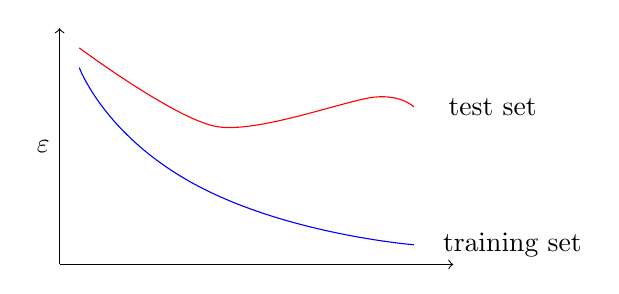
\begin{tikzpicture}
                        \draw
                        (0, 0) edge[->, left] node{$\varepsilon$} (0, 3)
                        (0, 0) edge[->] (5, 0);

                        \draw [red] plot [smooth] coordinates { (0.25, 2.75) (2, 1.75) (4, 2.125) (4.5, 2) };
                        \draw [blue] plot [smooth, tension=1] coordinates { (0.25, 2.5) (1.75, 1) (4.5, 0.25) };

                        \node at (5.5, 2) {test set};
                        \node at (5.75, 0.25) {training set};
                    \end{tikzpicture}
                \end{center}
                In the example above, it starts off with an underfitted model, and then ends up overfitted.
                The point where it's correct is just as the error of the test set begins to increase again.
                \medskip

                Overfitting can occur under these scenarios (and how we could avoid it);
                \begin{itemize}
                    \itemsep0em
                    \item model used is too complex (learns too many fine details)
                        \subitem use the validation set to decide the complexity
                    \item examples in the training set are not representative of all possible situations
                        \subitem obtain more data
                    \item learning is performed for too long (such as neural networks)
                        \subitem stopping the training earlier (using the validation set to decide when)
                \end{itemize}
            \subsubsection*{Confidence Intervals}
                The amount of data used in our test set also affects our confidence of the performance evaluation.
                A 90\% accuracy score on a test set with 10 samples is still less trustworthy than an 84\% accuracy score on a test set with 10,000 samples.
                \medskip

                We define the true error of the model $h$ as the probability that it will misclassify a randomly drawn example $x$ from distribution $D$;
                $$error_D(h) \equiv P[f(x) \neq h(x)]$$
                The \textbf{sample error} of the model $h$ based on a data sample $S$ is as follows;
                \begin{align*}
                    n & = \text{number of samples} \\
                    \delta(f(x), h(x)) & = \begin{cases}
                        1 & f(x) \neq h(x) \\
                        0 & f(x) = h(x)
                    \end{cases} \\
                    error_S(h) & \equiv \frac{1}{n} \summation{x \in S}{} \delta(f(x), h(x))
                \end{align*}
                We can say an $N\%$ confidence interval for some parameter $q$ is an interval with probability $N$ to contain the true value of $q$.
                Given a sample $S$, with more than 30 examples;
                $$error_S(h) \pm Z_N \underbrace{\sqrt{\frac{error_S(h) \cdot (1 - error_S(h))}{n}}}_\text{est. standard deviation of sample error}$$
                Due to the $n$ in the estimation of the standard deviation, if we have a very large $n$, we can obtain a very tight confidence interval.
                An example of this applied is as follows;
                \medskip

                Emotion recognition results for 3 samples, using 156 training and 50 testing samples.
                \begin{center}
                    \begin{tabular}{lllll}
                        & attributes & number of classes & classifier & correctly classified \\
                        \hline
                        face & 67 * 8 & C4.5 & 78\% \\
                        body & 140 & 6 & BayesNet & 90\%
                    \end{tabular}
                \end{center}
                We want to classify the 95\% confidence interval for this error ($Z_N = 1.96$)
                \begin{align*}
                    error_S(h) & = 0.22 \\
                    n & = 50 \\
                    Z_N & = 1.96 \\
                    \text{interval} & = \left[0.22 - 1.96\sqrt{\frac{0.22 \cdot (1 - 0.22)}{50}}, 0.22 + 1.96\sqrt{\frac{0.22 \cdot (1 - 0.22)}{50}}\right] \\
                    & = [0.11, 0.33]
                \end{align*}
            \subsubsection*{Significance Testing}
                Statistical tests can tell us if the means of two sets are significantly different;
                \begin{itemize}
                    \itemsep0em
                    \item \textbf{randomisation test}
                        \subitem
                            Randomly switch some predictions between two models and measure if the performance difference that we get is greater than or equal to the original difference.
                    \item \textbf{two-sample T-test}
                        \subitem
                            This is used to estimate if two metrics from different populations are actually different.
                            This has lower computational requirements and is easier to calculate.
                    \item \textbf{paired T-test}
                        \subitem
                            Examining significance over multiple matched results, such as classification error over the same folds in cross-validation.
                \end{itemize}
                The \textbf{null hypothesis} (see \textbf{CO245}) is the hypothesis that the two algorithms / models perform the same and the differences are only due to sampling error.
                These tests return a \textbf{p-value}, which is the probability of obtaining the differences we see, assuming the null hypothesis is correct.
                A small p-value implies that we can be more confident that one system is actually different.
                \medskip

                We consider a performance difference to be \textbf{statistically significant} of $p < 0.05$.
                However, $p > 0.05$ does not mean the algorithms are similar, just that we cannot observe a statistical difference.
                \medskip

                There's a fairly long bit on \textbf{P-hacking}, but not sure why.
                A way to protect against P-hacking is to use an adaptive p-value;
                \begin{enumerate}[1.]
                    \itemsep0em
                    \item rank p-values from $M$ experiments;
                        $$p_1 \leq p_2 \leq p_3 \leq \dots \leq p_M$$
                    \item calculate the \textbf{Benjamini-Hochberg} critical value for each experiment;
                        $$z_i = 0.05 \frac{i}{M}$$
                    \item significant results are the ones where the p-value is smaller than the critical value
                \end{enumerate}
        \subsection*{Week 5 (Artificial Neural Networks I)}
            \subsubsection*{The Rise of Neural Networks}
                \textbf{Artificial neural networks} are a class of machine learning algorithms, similar to \textbf{kNN} or \textbf{decision trees}.
                They consist of connected neurons, normally optimised with \textbf{gradient descent}.
                On the other hand \textbf{deep learning} refers to the use of neural network models with multiple hidden layers (hence deep) - they are usually trained on larger datasets for longer periods of time.
                \medskip

                Using neural network models, there was a large improvement in speech recognition.
                \textit{AlphaGo} allows for board analysis to beat human players (an exhaustive search isn't feasible compared to chess).
                Another example is realistic text generation, as well as video editing (see \textit{DeepFakes}) - automating what would take hours to do manually.
                The aforementioned example of video editing works by sharing an encoder, and feeding it to a decoder which specialises in generating a single face.
                To change a face, the encoded output from the first person is put into the decoder of the second.
                Another application is combining different information mediums (such as images and text) - for example generating descriptive outputs for a given image.
                \medskip

                The theory for neural networks had already existed (perceptrons in 1958, backpropagation in 1964, convolutional neural networks and LSTMs in the 1990s).
                However, today there is more data for training, as well as improved methods for storing and managing data.
                Similarly, neural networks benefit from faster hardware for computation (especially GPUs, since the matrix computation can be easily parallelised on GPUs).
                Finally, better software (such as automatic differentiation libraries) reduces the amount of work required (compared to manual calculation).
            \subsubsection*{Linear Regression}
                We can think of linear regression as a very simplified method of a neural network model.
                This is a form of \textbf{supervised learning}, where we assume we have a dataset of input and output pairs;
                \begin{itemize}
                    \itemsep0em
                    \item \textbf{dataset} \hfill $\{\la x^{(1)}, y^{1} \ra, \la x^{(N)}, y^{N} \ra, \dots, \la x^{(N)}, y^{N} \ra\}$
                    \item \textbf{input features} \hfill $X = \{x^{(1)}, x^{(2)}, \dots, x^{(N)}\}$
                    \item \textbf{known (desired) outputs} \hfill $Y = \{y^{(1)}, y^{(2)}, \dots, y^{(N)}\}$
                \end{itemize}
                Our aim is to learn the mapping $f : X \to Y$, such that $\forall i \in [1, N]\ f(x^{(i)}) = y^{(i)}$.
                In linear regression, $f$ is a linear function.
                \medskip

                It's important to note the difference between continuous and discrete problems;
                \begin{itemize}
                    \itemsep0em
                    \item \textbf{classification} \hfill desired labels are discrete
                        \begin{itemize}
                            \itemsep0em
                            \item obtaining digit labels from handwriting
                            \item obtaining sentiment from text
                        \end{itemize}
                    \item \textbf{regression} \hfill desired labels are continuous
                        \begin{itemize}
                            \itemsep0em
                            \item obtaining price of a house depending on some features
                            \item determining stock price from data on a company
                        \end{itemize}
                \end{itemize}
                An example of simple linear regression, with one input variable can be modelled as $y = ax + b$.
                $a$ denotes the slope, which controls the angle, $b$ denotes the intercept / bias (which controls the height) - with respect to a graph with the standard axes.
                \medskip

                Consider a dataset which contains GDP per capita ($x$) and enrolment rate ($y$).
                To find the best values for $a$ and $b$ in $\hat{y} = ax + b$, we must first determine what we mean by best.
            \subsubsection*{Loss Function}
                A loss / cost function determines how well we are doing on our dataset, where a smaller value of $E$ means our predictions are close to our real values.
                Consider the \textbf{sum-of-squares} loss function;
                \begin{align*}
                    E & = \frac{1}{2} \summation{i=1}{N} \left(\hat{y}^{(i)} - y^{(i)}\right)^2 \\
                    & = \frac{1}{2} \summation{i=1}{N} \left(ax^{(i)} + b - y^{(i)}\right)^2
                \end{align*}
                Note that the division by two is optional, however it allows for easier differentiation since it cancels with the two that will come from the square.
                By using a squared function, we are allowing for small errors that are close to the actual value, but we want to penalise the model for large errors.
            \subsubsection*{Updating Parameters with Derivatives}
                Working out the partial derivative of the previously mentioned loss function with respect to each of the parameters, we get the following;
                \begin{align*}
                    E & = \frac{1}{2} \summation{i=1}{N} \left(ax^{(i)} + b - y^{(i)}\right)^2 \\
                    \pdif{E}{a} & = \pdif{}{a} \frac{1}{2} \summation{i=1}{N} \left(ax^{(i)} + b - y^{(i)}\right)^2 \\
                    & = \frac{1}{2} \summation{i=1}{N} \pdif{}{a} \left(ax^{(i)} + b - y^{(i)}\right)^2 \\
                    & = \summation{i=1}{N} \left(ax^{(i)} + b - y^{(i)}\right) x^{(i)} \\
                    & = \summation{i=1}{N} \left(\hat{y}^{(i)} - y^{(i)}\right) x^{(i)} \\
                    \pdif{E}{b} & = \pdif{}{b} \frac{1}{2} \summation{i=1}{N} \left(ax^{(i)} + b - y^{(i)}\right)^2 \\
                    & = \frac{1}{2} \summation{i=1}{N} \pdif{}{b} \left(ax^{(i)} + b - y^{(i)}\right)^2 \\
                    & = \summation{i=1}{N} \left(ax^{(i)} + b - y^{(i)}\right) \\
                    & = \summation{i=1}{N} \left(\hat{y}^{(i)} - y^{(i)}\right)
                \end{align*}
            \subsubsection*{Gradient Descent}
                \textbf{Gradient descent} is the process of repeated updating our parameters by taking small steps (of learning rate / step size $\alpha$) in the negative direction of the partial derivative (worked out above).
                Note that we use $:=$ to denote a reassignment (not equality) in our \textbf{update rules}.
                \begin{align*}
                    a & := a - \alpha \pdif{E}{a} \\
                    & := a - \alpha \summation{i=1}{N} \left(\hat{y}^{(i)} - y^{(i)}\right) x^{(i)} \\
                    b & := b - \alpha \pdif{E}{b} \\
                    & := b - \alpha \summation{i=1}{N} \left(\hat{y}^{(i)} - y^{(i)}\right)
                \end{align*}
                This can be implemented manually as follows;
                \begin{lstlisting}
                    X = data["GDP"].values
                    Y = data["Enrolment Rate"].values

                    a = 0.0
                    b = 0.0
                    learning_rate = 1e-11

                    for epoch in range(5): # an epoch is a single iteration
                        update_a = 0.0
                        update_b = 0.0
                        error = 0.0
                        for i in range(len(Y)):
                            y_pred = a * X[i] + b
                            update_a += (y_predicted - Y[i]) * X[i]
                            update_b += (y_predicted - Y[i])
                            error += np.square(y_predicted - Y[i])

                        # Update rule for gradient descent
                        a = a - learning_rate * update_a
                        b = b - learning_rate * update_b

                        # the lines above can be shortened to the following
                        y_predicted = a * X + b
                        a = a - learning_rate * ((y_predicted - Y) * X).sum()
                        b = b - learning_rate * (y_predicted - Y).sum()
                        rmse = np.sqrt(np.square(y_predicted - Y).mean())
                \end{lstlisting}
                It can often be more convenient to work with vector notation.
                The gradient is a vector of all the partial derivatives.
                For a function $f : \mathbb{R}^K \to \mathbb{R}$ (where there are $K$ parameters) the gradient is;
                $$\nabla_\theta f(\theta) = \begin{bmatrix}
                    \pdif{f(\theta)}{\theta_1} \\
                    \pdif{f(\theta)}{\theta_2} \\
                    \vdots \\
                    \pdif{f(\theta)}{\theta_K}
                \end{bmatrix}$$
                Using this, there is an \textbf{analytical solution} for solving a single variable linear regression;
                \begin{align*}
                    \mat{X} & = \begin{bmatrix}
                        x^{(1)} & 1.0 \\
                        x^{(2)} & 1.0 \\
                        \vdots & \vdots \\
                        x^{(N)} & 1.0
                    \end{bmatrix} \\
                    \vec{y} & = \begin{bmatrix}
                        y^{(1)} \\ y^{(2)}\\ \vdots \\ y^{(N)}
                    \end{bmatrix} \\
                    \vec{\theta} & = \begin{bmatrix}
                        a \\ b
                    \end{bmatrix} \\
                    \nabla_\theta E(\vec{\theta}) & = \mat{X}^\top (\mat{X}\vec{\theta} - y) \\
                    & = 0 & \Rightarrow \\
                    \vec{\theta^*} & = (\mat{X}^\top\mat{X})^{-1}\mat{X}^\top\vec{y}
                \end{align*}
                While this requires no iteration to directly find the optimal parameter values, it's not great for large problems as the matrix inversion has cubic complexity.
                The analytical solution, presented here with \textit{Scikit-Learn}, has another benefit over gradient descent;
                \begin{lstlisting}
                    from sklearn.linear_model import LinearRegression

                    model = LinearRegression(fit_intercept=True)
                    X = data["GDP"].values.reshape(-1, 1)
                    Y = data["Enrolment Rate"]
                    model.fit(X, Y)

                    mse = np.square(Y - model.predict(X)).mean()
                \end{lstlisting}
                The analytical method manages to find the \textbf{global minimum}, whereas gradient descent finds a \textbf{local minimum}.
            \subsubsection*{Multiple Linear Regression}
                The previous example only took into account a single feature, which likely is insufficient for most complex problems.
                \textbf{multiple linear regression} considers many input features as follows, where \violet{each input feature has its own parameter} as well as an \teal{extra parameter which acts as a bias};
                \begin{center}
                    $y^{(i)} = \violet{\summation{j=1}{K} \theta_j x^{(i)}_j} + \teal{\theta_{K + 1}}$
                \end{center}
                Note that compared to before, when this is graphed on a two dimensional plane, it will be discontinuous, as it will exist in higher dimensions.
            \subsubsection*{Artificial Neuron}
                In the example below, we have the \textbf{features} $x_i$ and a corresponding weight (\textbf{parameter}) $\theta_i$.
                \begin{center}
                    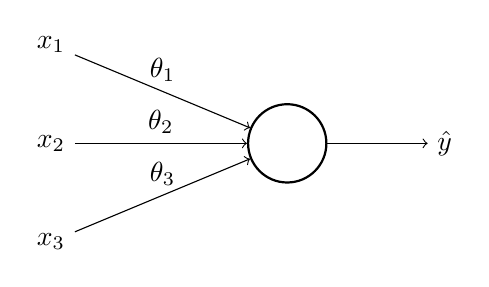
\begin{tikzpicture}[x=2cm, y=1.25cm]
                        \node (x1) at (-1.5, 1) {$x_1$};
                        \node (x2) at (-1.5, 0) {$x_2$};
                        \node (x3) at (-1.5, -1) {$x_3$};
                        \node[inner sep=10pt, circle, draw=black, thick] (n) at (0, 0) {};
                        \node (yh) at (1, 0) {$\hat{y}$};

                        \draw
                        (x1) edge[->, above] node{$\theta_1$} (n)
                        (x2) edge[->, above] node{$\theta_2$} (n)
                        (x3) edge[->, above] node{$\theta_3$} (n)
                        (n) edge[->] (yh);
                    \end{tikzpicture}
                \end{center}
                The output value of the neuron above is as follows, where $g$ is the \textbf{activation function} (this is what makes it a neuron instead of just linear regression) and $b$ is the \textbf{bias};
                \begin{center}
                    $\hat{y} = g(\underbrace{\theta_1 x_1 + \theta_2 x_2 + \theta_3 x_3 + b}_\text{linear regression})$
                \end{center}
                Note that the bias is often implicit, since we can simply add an extra input feature that has a value of 1.
                Note that it's also possible to represent the weights as a vector $\vec{W}$, which simplifies the equation to be the following;
                \begin{center}
                    $\hat{y} = g(\vec{W}^\top\vec{x})$
                \end{center}
                Note that the part inside the activation function, concerning $W$ and $x$, can be written in any way (depending on the representation), as long as the dimensions line up to give a single scalar result.
            \subsubsection*{Logistic Activation Function}
                The \textbf{logistic function} is also known as the \textbf{sigmoid function};
                \begin{align*}
                    g(z) & = \frac{1}{1 + e^{-z}} \\
                    z & \in \mathbb{R} \\
                    \hat{y} & \in [0, 1]
                \end{align*}
                \begin{center}
                    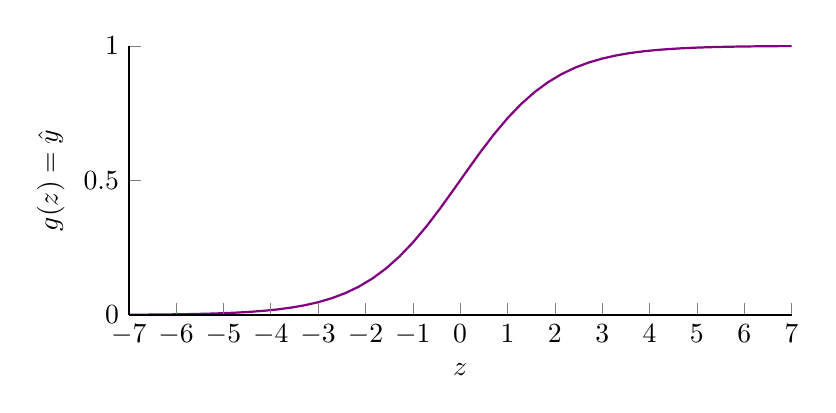
\begin{tikzpicture}
                        \begin{axis}[
                            axis on top=true,
                            axis line style=thick,
                            no markers, domain=-7:7, samples=50,
                            axis lines*=left, xlabel=$z$, ylabel=${g(z) = \hat{y}}$,
                            height=5cm, width=10cm,
                            enlargelimits=false,
                            xtick={-7,-6,...,7},
                            ytick={0,0.5,1},
                            xmin=-7, xmax=7,
                            ymin=0, ymax=1
                        ]
                            \addplot[violet, thick] {1 / (1 + exp(-1 * \x))};
                        \end{axis}
                    \end{tikzpicture}
                \end{center}
                In logistic regression (which actually isn't regression), we can pass the output of linear regression through a logistic function, allowing us to get either 0 or 1 (binary classification).
                The model is optimised using gradient descent.
            \subsubsection*{Perceptron}
                This is another algorithm for supervised binary classification (similarly has the two classes 0 and 1).
                It uses a threshold function as the activation function;
                $$h(x) = f(\vec{W}^\top\vec{x}) = \begin{cases}
                    1 & \text{if } \vec{W}^\top\vec{x} > 0 \\
                    0 & \text{otherwise}
                \end{cases}$$
                The learning rule is as follows;
                \begin{center}
                    $\theta_i \leftarrow \theta_i + \alpha(y - h(x))x_i$
                \end{center}
                The reasoning is as follows; if the desired output ($y$) is equal to our prediction ($h(x)$), then the right hand side of the summation becomes 0, thus the parameter is unchanged - we don't fix it if it isn't broken.
                On the other hand, if the true value is 1 and the prediction is 0, we want to make $\vec{W}^\top\vec{x}$ bigger since the desired output is bigger than our prediction (therefore our prediction is too small to be set to 1 by the activation function).
                Since $y - h(x) = 1$ in this case, we increase $\theta_i$ if $x_i$ is positive, and decrease it if it is negative.
                The reasoning holds the other way around, when the true value is 0 but we predict 1.
                \medskip

                Any linearly separable function can be learnt with a perceptron, such as logical ~OR~ or ~AND~, however something like ~XOR~ cannot be learnt.
                The activation function is also very sharp (and also not differentiable) so it's not used in most complex neural networks.
            \subsubsection*{Connecting Neurons}
                We can connect multiple neurons in parallel and consider each one as a \textbf{feature detector};
                \begin{center}
                    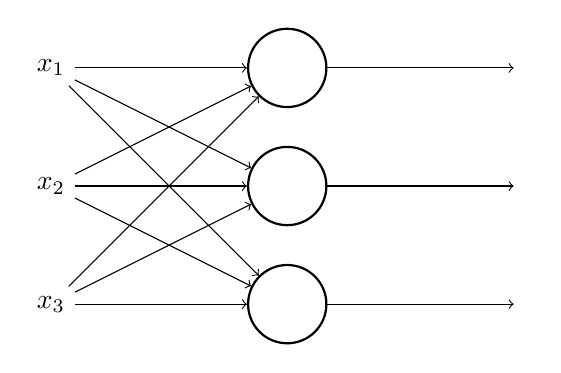
\begin{tikzpicture}[x=3cm, y=1.5cm]
                        \node (x1) at (-1, 1) {$x_1$};
                        \node (x2) at (-1, 0) {$x_2$};
                        \node (x3) at (-1, -1) {$x_3$};
                        \node[inner sep=10pt, circle, draw=black, thick] (n1) at (0, 1) {};
                        \node[inner sep=10pt, circle, draw=black, thick] (n2) at (0, 0) {};
                        \node[inner sep=10pt, circle, draw=black, thick] (n3) at (0, -1) {};
                        \node (o1) at (1, 1) {};
                        \node (o2) at (1, 0) {};
                        \node (o3) at (1, -1) {};

                        \draw
                        (x1) edge[->] (n1)
                        (x1) edge[->] (n2)
                        (x1) edge[->] (n3)
                        (x2) edge[->] (n1)
                        (x2) edge[->] (n2)
                        (x2) edge[->] (n3)
                        (x3) edge[->] (n1)
                        (x3) edge[->] (n2)
                        (x3) edge[->] (n3)
                        (n1) edge[->] (o1)
                        (n2) edge[->] (o2)
                        (n3) edge[->] (o3);
                    \end{tikzpicture}
                \end{center}
                Similarly, we can connect neurons in sequence to learn from higher-order features (this is a multilayer perceptron, which isn't actually a perceptron);
                \begin{center}
                    \begin{tikzpicture}[x=3cm, y=1.5cm]
                        \node (x1) at (-1, 1) {$x_1$};
                        \node (x2) at (-1, 0) {$x_2$};
                        \node (x3) at (-1, -1) {$x_3$};
                        \node[inner sep=10pt, circle, draw=black, thick] (n11) at (0, 1) {};
                        \node[inner sep=10pt, circle, draw=black, thick] (n12) at (0, 0) {};
                        \node[inner sep=10pt, circle, draw=black, thick] (n13) at (0, -1) {};
                        \node[inner sep=10pt, circle, draw=black, thick] (n21) at (1, 1) {};
                        \node[inner sep=10pt, circle, draw=black, thick] (n22) at (1, 0) {};
                        \node[inner sep=10pt, circle, draw=black, thick] (n23) at (1, -1) {};
                        \node (o1) at (2, 1) {};
                        \node (o2) at (2, 0) {};
                        \node (o3) at (2, -1) {};

                        \draw
                        (x1) edge[->] (n1)
                        (x1) edge[->] (n2)
                        (x1) edge[->] (n3)
                        (x2) edge[->] (n1)
                        (x2) edge[->] (n2)
                        (x2) edge[->] (n3)
                        (x3) edge[->] (n1)
                        (x3) edge[->] (n2)
                        (x3) edge[->] (n3)
                        (n11) edge[->] (n21)
                        (n11) edge[->] (n22)
                        (n11) edge[->] (n23)
                        (n12) edge[->] (n21)
                        (n12) edge[->] (n22)
                        (n12) edge[->] (n23)
                        (n13) edge[->] (n21)
                        (n13) edge[->] (n22)
                        (n13) edge[->] (n23)
                        (n21) edge[->] (o1)
                        (n22) edge[->] (o2)
                        (n23) edge[->] (o3);
                    \end{tikzpicture}
                \end{center}
                A multilayer perceptron with a sufficient number of neurons can theoretically model an arbitrary function over an input.
                However, drawing this can be tedious (and isn't even feasible for large networks), we can represent each layer as a block, and each fully connected matrix of weights as an arrow (the diagram below represents the diagram above);
                \begin{center}
                    \begin{tikzpicture}[x=3cm, y=1.5cm]
                        \draw (-1.25, 1.25) -- (-0.75, 1.25) -- (-0.75, -1.25) -- (-1.25, -1.25) -- cycle;
                        \node at (-1, 0) {$x$};
                        \draw (-0.25, 1.25) -- (0.25, 1.25) -- (0.25, -1.25) -- (-0.25, -1.25) -- cycle;
                        \node at (0, 0) {$h_1$};
                        \draw (0.75, 1.25) -- (1.25, 1.25) -- (1.25, -1.25) -- (0.75, -1.25) -- cycle;
                        \node at (1, 0) {$h_2$};

                        \draw
                        (-0.75, 0) edge[->] (-0.25, 0)
                        (0.25, 0) edge[->] (0.75, 0)
                        (1.25, 0) edge[->] (2, 0);
                    \end{tikzpicture}
                \end{center}
                We typically refer to the first layer as the \textbf{input layer}, the final layer as the \textbf{output layer}, and everything in between the two as \textbf{hidden layers}.
                Consider a network with an input layer $x$, an output layer $\hat{y}$, and a hidden layer $h$;
                \begin{center}
                    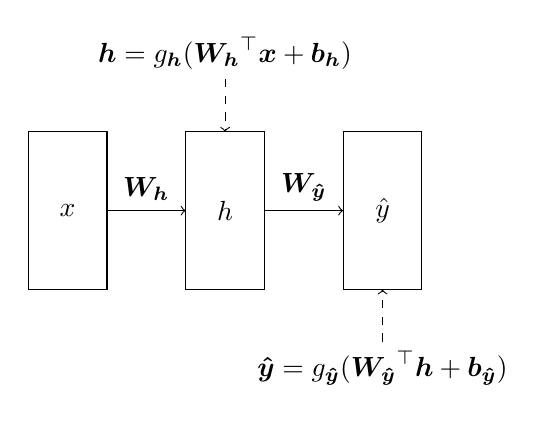
\begin{tikzpicture}
                        \draw (0, 0) -- (1, 0) -- (1, -2) -- (0, -2) -- cycle;
                        \node at (0.5, -1) {$x$};
                        \draw (2, 0) -- (3, 0) -- (3, -2) -- (2, -2) -- cycle;
                        \node at (2.5, -1) {$h$};
                        \draw (4, 0) -- (5, 0) -- (5, -2) -- (4, -2) -- cycle;
                        \node at (4.5, -1) {$\hat{y}$};

                        \node (he) at (2.5, 1) {$\vec{h} = g_{\vec{h}}(\vec{W_h}^\top \vec{x} + \vec{b_h})$};
                        \node (ye) at (4.5, -3) {$\vec{\hat{y}} = g_{\vec{\hat{y}}}(\vec{W_{\hat{y}}}^\top \vec{h} + \vec{b_{\hat{y}}})$};

                        \draw
                        (he) edge[->, dashed] (2.5, 0)
                        (ye) edge[->, dashed] (4.5, -2)
                        (1, -1) edge[->, above] node{$\vec{W_h}$} (2, -1)
                        (3, -1) edge[->, above] node{$\vec{W_{\hat{y}}}$} (4, -1);
                    \end{tikzpicture}
                \end{center}
                When something doesn't work, it's often a good idea to verify the dimensions match up (possibly missing a transpose);
                \begin{align*}
                    \vec{x} & \in \mathbb{R}^{K \times 1} \\
                    \vec{h} & \in \mathbb{R}^{H \times 1} \\
                    \vec{W_h} & \in \mathbb{R}^{K \times H} \\
                    \vec{b_h} & \in \mathbb{R}^{H \times 1} \\
                    \vec{\hat{y}} & \in \mathbb{R}^{C \times 1} \\
                    \vec{W_{\hat{y}}} & \in \mathbb{R}^{H \times C} \\
                    \vec{b_{\hat{y}}} & \in \mathbb{R}^{C \times 1}
                \end{align*}
            \subsubsection*{Learning Representations and Features}
                It's also important to note the difference between traditional pattern recognition and end-to-end training.
                For example with image recognition, traditional pattern recognition would require someone to manually craft a feature extractor, which then goes into a trainable classifier to give an output.
                This is in contrast to end-to-end training, where useful features are learnt from the data and trained with the classifier.
                This is useful as the feature extractor (typically at the lower levels of the network) can change to help the higher levels of the network make better decisions.
                \medskip

                For example (at a very abstract level), a face detector would be structured as follows - note how the lower levels generally learn individual features, and the higher levels learn features of the features from lower levels);
                \begin{itemize}
                    \itemsep0em
                    \item initially works on individual pixels
                    \item detects edges
                    \item detects components of a face
                    \item detects full faces
                \end{itemize}
            \subsubsection*{Activation Functions}
                If we are able to use a linear model to capture all the features of our data, then we should do so (use the simplest model we can).
                However, more likely than not, our data will not be linearly separable, and therefore complex patterns cannot be captured with linear models.
                For multilayer networks, activation functions become more important.
                \begin{itemize}
                    \itemsep0em
                    \item \textbf{linear activation} \hfill equivalent to having no activation function
                        $$f(x) = x$$
                        We cannot only use linear activation as multi-layer linear networks are equivalent to a single layer;
                        \begin{align*}
                            \mat{U} & = \mat{W_1}\mat{W_2} \\
                            \vec{\hat{y}} & = \mat{W_1}(\mat{W_2}\vec{x}) \\
                            & = \mat{U}\vec{x} & \text{becomes a single layer}
                        \end{align*}
                    \item \violet{\textbf{sigmoid activation}} \hfill smoothly compresses the output into $[0, 1]$
                        $$f(x) = \sigma(x) = \frac{1}{1 + e^{-x}}$$
                    \item \teal{\textbf{tanh activation}} \hfill similar shape to sigmoid, but range in $[-1, 1]$
                        $$f(x) = \tanh(x) = \frac{e^x - e^{-x}}{e^x + e^{-x}}$$
                    \item \blue{\textbf{ReLU activation}} \hfill rectified linear unit (linear in positive part)
                        $$f(x) = \text{ReLU}(x) = \begin{cases}
                            0 & \text{if } x \leq 0 \\
                            x & \text{otherwise}
                        \end{cases} = \max(0, x)$$
                    \item \textbf{softmax activation}
                        \subitem scales inputs into a probability distribution (largest will be large, rest small), all output values sum to 1
                        $$\text{softmax}(z_i) = \frac{e^{z_i}}{\summation{k}{} e^{z_k}}$$
                        This acts as a differentiable version of the max function, as it pushes the highest values close to 1 and the lower (remaining) values to 0.
                        It identifies the value with the highest confidence and assigns more probability to it - very useful for image classification.
                \end{itemize}
                We can see the functions graphically as follows;
                \begin{center}
                    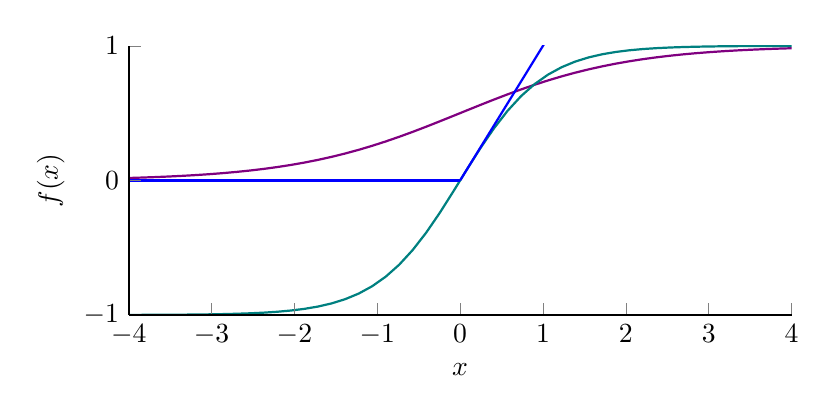
\begin{tikzpicture}
                        \begin{axis}[
                            axis on top=true,
                            axis line style=thick,
                            no markers, domain=-4:4, samples=50,
                            axis lines*=left, xlabel=$x$, ylabel=$f(x)$,
                            height=5cm, width=10cm,
                            enlargelimits=false,
                            xtick={-4,-3,...,4},
                            ytick={-1,0,1},
                            xmin=-4, xmax=4,
                            ymin=-1, ymax=1
                        ]
                            \addplot[violet, thick] {1 / (1 + exp(-1 * \x))};
                            \addplot[teal, thick] {tanh(\x)};
                            \addplot[blue, thick, domain=-4:0] {0};
                            \addplot[blue, thick, domain=0:4] {\x};
                        \end{axis}
                    \end{tikzpicture}
                \end{center}
                Note that most activation functions are applied \textbf{element-wise}, where each element is passed through the function independently (with the exception of softmax).
                \medskip

                ReLU is used commonly for very deep networks, however tanh and sigmoid also work well and can be argued to be more robust.
                Those functions are more robust as ReLU is unbounded (if something is broken in the network, ReLU will give a large value which leads to more problems in the higher levels of the network).
                Therefore, the activation functions used are also a hyperparameter.
                The activation of the output layer should depend on the task (since it determines what the model can actually output);
                \begin{itemize}
                    \itemsep0em
                    \item classifying into two classes \hfill sigmoid or tanh
                    \item predicting an unbounded score \hfill linear
                    \item predicting a probability distribution \hfill softmax
                \end{itemize}
            \subsubsection*{Feedforward Network in PyTorch}
                \begin{lstlisting}
                    import torch
                    import torch.nn as nn

                    class Net(nn.Module):
                        def __init__(self):
                            super(Net, self).__init__()
                            self.layer_h = nn.Linear(10, 5) # input->hidden (input of size 10)
                            self.layer_y = nn.Linear(5, 1) # hidden->output (hidden layer of size 5, gives 1 output)

                        def forward(self, x):
                            h = torch.tanh(self.layer_h(x)) # hidden layer with tanh activation
                            y = torch.sigmoid(self.layer_y(h)) # output with sigmoid activation

                    net = Net()
                    input = torch.FloatTensor([x for x in range(10)]) # sample input
                    output = net(input) # execution
                \end{lstlisting}
        \subsection*{Week 6 (Artificial Neural Networks II)}
            \subsubsection*{Loss Functions}
                We need to define a loss function which we aim to minimise, a smaller loss function tells us that we are doing better on a particular task.
                To optimise a neural network, we want to iteratively update parameters with gradient descent (taking small steps in the negative direction of the loss function), aiming to reduce the loss function.
                The general formula is as follows;
                $$\theta^{(t + 1)}_i = \theta^{(t)}_i - \alpha \pdif{E}{\theta^{(t)}_i}$$
            \subsubsection*{Loss Function for Regression}
                When we aim to predict a continuous variable, we often use linear activation (to avoid restricting the output).
                This is also often optimised with \textbf{mean squared error} (or quadratic / L2 loss).
                $$\text{MSE} = \frac{1}{N} \summation{i=1}{N} \left(\hat{y}_i - y_i\right)^2$$
                If the value is 0, then we know that our predictions are equal to our target data.
            \subsubsection*{Loss Function for Classification}
                In contrast, for classification the model needs to choose between discrete (categorical) options;
                \begin{itemize}
                    \itemsep0em
                    \item \textbf{binary classification} \hfill one of two possible choices (e.g. disease diagnosis)
                    \item \textbf{multi-class classification} \hfill an object can take one of many classes (e.g. detecting digits)
                    \item \textbf{multi-label classification} \hfill an object can take multiple classes (e.g. detecting objects in an image)
                \end{itemize}
                In \textbf{cross-entropy}, we aim to maximise the likelihood of the network assigning the correct labels to all the inputs in our dataset;
                $$\product{i=1}{N}P(y^{(i)}\ |\ x^{(i)}; \theta)$$
                Also assume that the examples are independent and identically distributed;
                $$P(A \land B) = P(A)P(B)$$
                For binary classification, we can consider the output of the network as a parameter of a \textbf{Bernoulli distribution};
                $$\product{i=1}{N} \left(\hat{y}^{(i)}\right)^{y^{(i)}}\left(1 - \hat{y}^{(i)}\right)^{\left(1 - y^{(i)}\right)}$$
                If we always correctly assign all the probability to the correct label, we end up with an output of 1, and if we always incorrectly assign the probability we get 0.
                \medskip

                However, dealing with multiplication of small values (since all of our values will be between 0 and 1) can lead to rounding errors in computers, we want to take logarithms.
                Since maximising the logarithm is identical;
                $$\summation{i=1}{N} y^{(i)}\log\left(\hat{y}^{(i)}\right) + \left(1 - y^{(i)}\right)\log\left(1 - \hat{y}^{(i)}\right)$$
                This can be turned into a loss (\textbf{binary cross-entropy}), which we aim to minimise.
                The division by $N$ is optional, but it avoids the magnitude of the loss being affected by the number of datapoints;
                $$L = -\frac{1}{N}\summation{i=1}{N} (\underbrace{y^{(i)}\log\left(\hat{y}^{(i)}\right)}_\text{class 1} + \underbrace{\left(1 - y^{(i)}\right)\log\left(1 - \hat{y}^{(i)}\right)}_\text{class 0})$$
                Notice that the above refers to two distinct classes - we can generalise this to multiple classes in \textbf{categorical cross-entropy};
                $$L = -\frac{1}{N}\summation{i=1}{N} \summation{c=1}{C} y^{(i)}_c\log\left(\hat{y}^{(i)}_c\right)$$
                Here $C$ is the set of possible classes, and $\hat{y}^{(i)}_c$ is the predicted probability of class $c$ for datapoint $i$.
                \medskip

                For multi-class classification, it's common to use softmax activation with categorical cross-entropy loss.
                Some examples are as follows;
                \begin{center}
                    \begin{tabular}{|l|l|l|l|}
                        \hline
                        \textbf{problem} & \textbf{type} & \textbf{output activation} & \textbf{loss} \\
                        \hline
                        future stock prices & regression & linear & MSE \\
                        stock prices up or down & binary & sigmoid & binary cross-entropy \\
                        speech recognition & multi-class & softmax & categorical cross-entropy \\
                        chemical properties & multi-label & sigmoid & binary cross-entropy \\
                        \hline
                    \end{tabular}
                \end{center}
                Note that for the final example, the activation is sigmoid for \textbf{each} individual output and we optimise each output with binary cross-entropy (such that each output acts as its own binary classifier for that property).
            \subsubsection*{Batching}
                A common process is to combine the vectors of several datapoints into one matrix to improve speed and reduce noise.
                The speed improvement comes from GPUs being able to handle parallel workloads such as matrix multiplication well, whereas more time will be spent copying vectors to the GPU without batching.
                See the example below where datapoint 1 ($x_{1, i}$) and datapoint 2 ($x_{2, i}$) are multiplied by the same weight matrix;
                \begin{align*}
                    \begin{bmatrix}
                        \blue{x_{1, 1}} & \blue{x_{1, 2}}
                    \end{bmatrix} \begin{bmatrix}
                        w_{1, 1} & w_{1, 2} & w_{1, 3} \\
                        w_{2, 1} & w_{2, 2} & w_{2, 3}
                    \end{bmatrix} & = \begin{bmatrix}
                        \teal{x_{1, 1}w_{1, 1} + x_{1, 2}w_{2, 1}} & \teal{x_{1, 1}w_{1, 2} + x_{1, 2}w_{2, 2}} & \teal{x_{1, 1}w_{1, 3} + x_{1, 2}w_{2, 3}}
                    \end{bmatrix} \\
                    \begin{bmatrix}
                        \red{x_{2, 1}} & \red{x_{2, 2}}
                    \end{bmatrix} \begin{bmatrix}
                        w_{1, 1} & w_{1, 2} & w_{1, 3} \\
                        w_{2, 1} & w_{2, 2} & w_{2, 3}
                    \end{bmatrix} & = \begin{bmatrix}
                        \violet{x_{2, 1}w_{1, 1} + x_{2, 2}w_{2, 1}} & \violet{x_{2, 1}w_{1, 2} + x_{2, 2}w_{2, 2}} & \violet{x_{2, 1}w_{1, 3} + x_{2, 2}w_{2, 3}}
                    \end{bmatrix} \\
                    \begin{bmatrix}
                        \blue{x_{1, 1}} & \blue{x_{1, 2}} \\
                        \red{x_{2, 1}} & \red{x_{2, 2}}
                    \end{bmatrix} \begin{bmatrix}
                        w_{1, 1} & w_{1, 2} & w_{1, 3} \\
                        w_{2, 1} & w_{2, 2} & w_{2, 3}
                    \end{bmatrix} & = \begin{bmatrix}
                        \teal{x_{1, 1}w_{1, 1} + x_{1, 2}w_{2, 1}} & \teal{x_{1, 1}w_{1, 2} + x_{1, 2}w_{2, 2}} & \teal{x_{1, 1}w_{1, 3} + x_{1, 2}w_{2, 3}} \\
                        \violet{x_{2, 1}w_{1, 1} + x_{2, 2}w_{2, 1}} & \violet{x_{2, 1}w_{1, 2} + x_{2, 2}w_{2, 2}} & \violet{x_{2, 1}w_{1, 3} + x_{2, 2}w_{2, 3}}
                    \end{bmatrix}
                \end{align*}
                This method is applied to the majority of neural network operations, such as addition, subtraction as well as application of activation functions.
            \subsubsection*{Forward and Backward Pass}
                The following process applies from the bottom up ($X$ progresses to $\hat{Y}$);
                \begin{align*}
                    \text{Loss} & = L(Y, \hat{Y}) \\
                    \hat{Y} & = g_{o}\left(Z^{[3]}\right) \\
                    Z^{[3]} & = A^{[2]}W^{[3]} + B^{[3]} \\
                    A^{[2]} & = g_{h_2}\left(Z^{[2]}\right) \\
                    Z^{[2]} & = A^{[1]}W^{[2]} + B^{[2]} \\
                    A^{[1]} & = g_{h_1}\left(Z^{[1]}\right) \\
                    Z^{[1]} & = XW^{[1]} + B^{[1]} \\
                    X & \in \mathbb{R}^{N \times K} & \text{$N$ datapoints and $K$ features per datapoint}
                \end{align*}
                The idea of backpropagation reduces the work needed by splitting up the workload for calculating partial derivatives.
                The partial derivative is obtained by using the partial derivative from the next layer (the next layer in the forward pass), which obtains it from the partial derivative of the loss function.
                \begin{center}
                    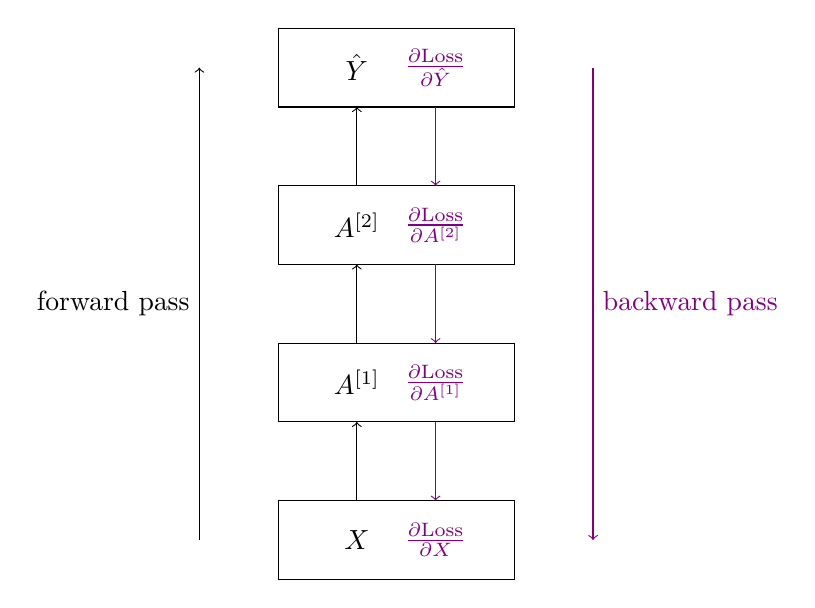
\begin{tikzpicture}
                        \draw (0, 0) -- (3, 0) -- (3, -1) -- (0, -1) -- cycle;
                        \draw (0, -2) -- (3, -2) -- (3, -3) -- (0, -3) -- cycle;
                        \draw (0, -4) -- (3, -4) -- (3, -5) -- (0, -5) -- cycle;
                        \draw (0, -6) -- (3, -6) -- (3, -7) -- (0, -7) -- cycle;

                        \node at (1, -0.5) {$\hat{Y}$};
                        \node at (1, -2.5) {$A^{[2]}$};
                        \node at (1, -4.5) {$A^{[1]}$};
                        \node at (1, -6.5) {$X$};

                        \node at (2, -0.5) {$\violet{\pdif{\text{Loss}}{\hat{Y}}}$};
                        \node at (2, -2.5) {$\violet{\pdif{\text{Loss}}{A^{[2]}}}$};
                        \node at (2, -4.5) {$\violet{\pdif{\text{Loss}}{A^{[1]}}}$};
                        \node at (2, -6.5) {$\violet{\pdif{\text{Loss}}{X}}$};

                        \draw
                        (-1, -6.5) edge[->, left] node{forward pass} (-1, -0.5)
                        (4, -6.5) edge[<-, right, violet] node{backward pass} (4, -0.5)
                        (1, -6) edge[->] (1, -5)
                        (1, -4) edge[->] (1, -3)
                        (1, -2) edge[->] (1, -1)
                        (2, -6) edge[<-, violet] (2, -5)
                        (2, -4) edge[<-, violet] (2, -3)
                        (2, -2) edge[<-, violet] (2, -1);
                    \end{tikzpicture}
                \end{center}
                By recalling the \textbf{chain rule} (for calculating derivatives of composite functions);
                \begin{align*}
                    z & = f(x) \\
                    y & = g(z) \\
                    \dif{y}{x} & = \dif{y}{z} \cdot \dif{z}{x}
                \end{align*}
                For example, assume we want to find the partial derivative with respect to the weight matrix $W^{[1]}$ (which we would want to do for gradient descent).
                We can break down our derivatives as follows;
                \begin{align*}
                    \pdif{\text{Loss}}{Z^{[1]}} & = \pdif{\text{Loss}}{A^{[1]}} \cdot \pdif{A^{[1]}}{Z^{[1]}} \\
                    \pdif{\text{Loss}}{W^{[1]}} & = \pdif{\text{Loss}}{Z^{[1]}} \cdot \pdif{Z^{[1]}}{W^{[1]}} \\
                    & = \pdif{\text{Loss}}{\hat{Y}} \cdot \teal{\pdif{\hat{Y}}{Z^{[3]}}} \cdot \violet{\pdif{Z^{[3]}}{A^{[2]}}} \cdot \teal{\pdif{A^{[2]}}{Z^{[2]}}} \cdot \violet{\pdif{Z^{[2]}}{A^{[1]}}} \cdot \teal{\pdif{A^{[1]}}{Z^{[1]}}} \cdot \pdif{Z^{[1]}}{W^{[1]}}
                \end{align*}
                We can see the partial derivatives in \teal{teal} are the output of an activation function with respect to the inputs, whereas the ones in \violet{violet} are the output of a linear transformation with respect to the input of a linear transformation.
                We cannot directly apply this on matrices, as they are 4D tensors.
                \begin{center}
                    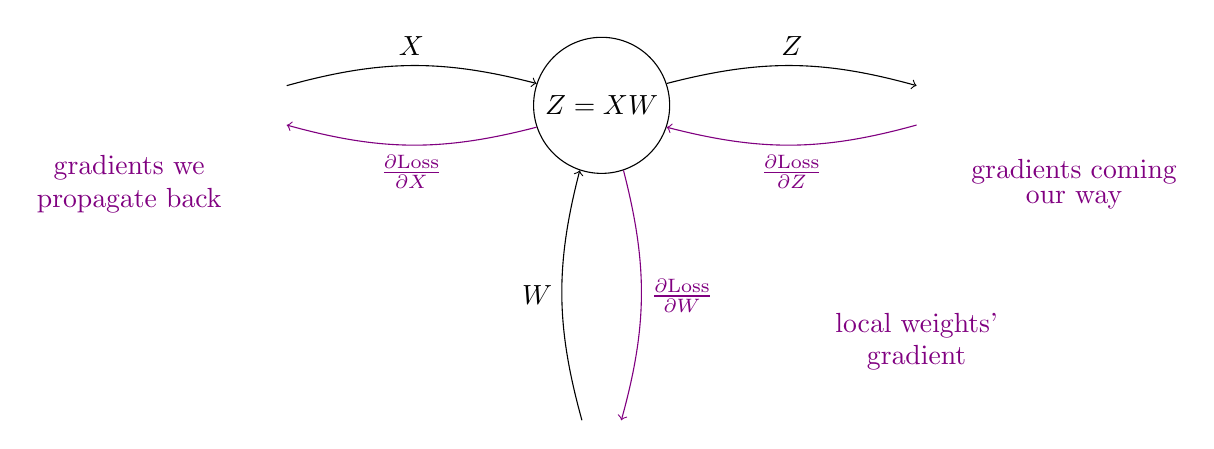
\begin{tikzpicture}
                        \node[draw, circle] (o) at (0, 0) {$Z = XW$};

                        \node[violet] at (-6, -1) {\shortstack{gradients we\\propagate back}};
                        \node[violet] at (6, -1) {\shortstack{gradients coming\\our way}};
                        \node[violet] at (4, -3) {\shortstack{local weights'\\gradient}};

                        \draw
                        (-4, 0.25) edge[->, bend left=15, above] node{$X$} (o)
                        (-4, -0.25) edge[<-, bend right=15, below, violet] node{$\pdif{\text{Loss}}{X}$} (o)
                        (o) edge[->, bend left=15, above] node{$Z$} (4, 0.25)
                        (o) edge[<-, bend right=15, below, violet] node{$\pdif{\text{Loss}}{Z}$} (4, -0.25)
                        (-0.25, -4) edge[->, bend left=15, left] node{$W$} (o)
                        (0.25, -4) edge[<-, bend right=15, right, violet] node{$\pdif{\text{Loss}}{W}$} (o);
                    \end{tikzpicture}
                \end{center}
                \begin{align*}
                    X & \in \mathbb{R}^{N \times D} \\
                    W & \in \mathbb{R}^{D \times M} \\
                    B & \in \mathbb{R}^{N \times M} \\
                    Z & \in \mathbb{R}^{N \times M} \\
                    Z & = XW + B \\
                    \intertext{consider a particular case, where;}
                    N & = 2 \\
                    D & = 2 \\
                    M & = 3 \\
                    X & = \begin{bmatrix}
                        x_{1, 1} & x_{1, 2} \\
                        x_{2, 1} & x_{2, 2}
                    \end{bmatrix} \\
                    W & = \begin{bmatrix}
                        w_{1, 1} & w_{1, 2} & w_{1, 3} \\
                        w_{2, 1} & w_{2, 2} & w_{2, 3}
                    \end{bmatrix} \\
                    B & = \begin{bmatrix}
                        \vec{b} \\ \vec{b}
                    \end{bmatrix} & \text{same bias} \\
                    & = \begin{bmatrix}
                        b_1 & b_2 & b_3 \\
                        b_1 & b_2 & b_3
                    \end{bmatrix} \\
                    Z & = \begin{bmatrix}
                        x_{1, 1}w_{1, 1} + x_{1, 2}w_{2, 1} + b_1 & x_{1, 1}w_{1, 2} + x_{1, 2}w_{2, 2} + b_2 & x_{1, 1}w_{1, 3} + x_{1, 2}w_{2, 3} + b_3 \\
                        x_{2, 1}w_{1, 1} + x_{2, 2}w_{2, 1} + b_1 & x_{2, 1}w_{1, 2} + x_{2, 2}w_{2, 2} + b_2 & x_{2, 1}w_{1, 3} + x_{2, 2}w_{2, 3} + b_3
                    \end{bmatrix} \\
                    \intertext{assume we already receive the following through backpropagation (notice it has the same shape as $Z$ - generally the derivative of a scalar with respect to a matrix has the same shape as the matrix)}
                    \pdif{\text{Loss}}{Z} & = \begin{bmatrix}
                        \pdif{\text{Loss}}{z_{1, 1}} & \pdif{\text{Loss}}{z_{1, 2}} & \pdif{\text{Loss}}{z_{1, 3}} \\
                        \pdif{\text{Loss}}{z_{2, 1}} & \pdif{\text{Loss}}{z_{2, 2}} & \pdif{\text{Loss}}{z_{2, 3}}
                    \end{bmatrix} \\
                    \intertext{to update weights, we need to calculate the following;}
                    \pdif{\text{Loss}}{W} & = \pdif{\text{Loss}}{Z} \cdot \pdif{Z}{W} \\
                    \pdif{\text{Loss}}{b} & = \pdif{\text{Loss}}{Z} \cdot \pdif{Z}{b} \\
                    \intertext{the following is needed to pass the gradient on to the lower layer;}
                    \pdif{\text{Loss}}{X} & = \pdif{\text{Loss}}{Z} \cdot \pdif{Z}{X}
                \end{align*}
                Looking at calculating this for a single value, we can visualise it as follows;
                \begin{center}
                    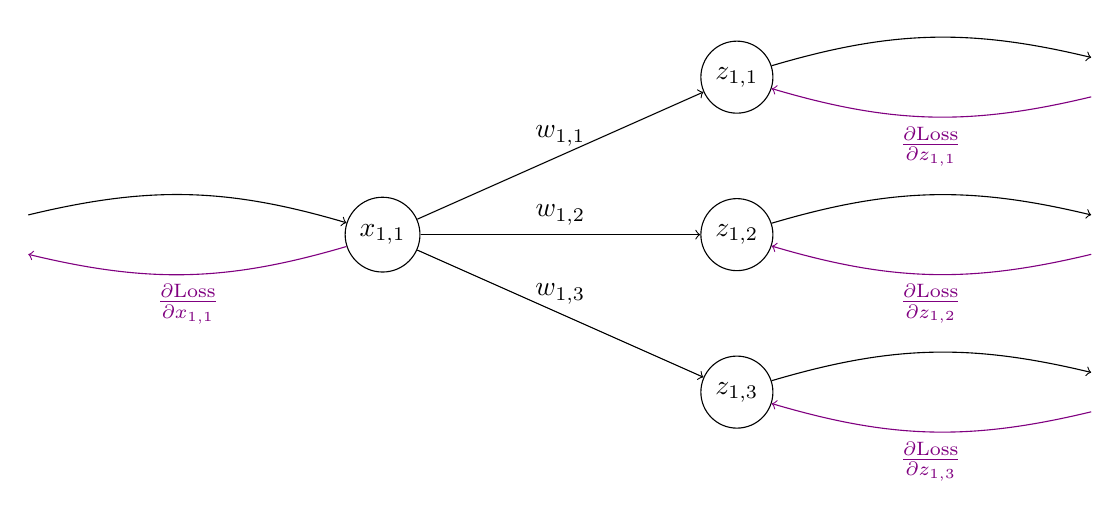
\begin{tikzpicture}[x=1.5cm]
                        \node[draw, circle] (x) at (0, 0) {$x_{1, 1}$};
                        \node[draw, circle] (z1) at (3, 2) {$z_{1, 1}$};
                        \node[draw, circle] (z2) at (3, 0) {$z_{1, 2}$};
                        \node[draw, circle] (z3) at (3, -2) {$z_{1, 3}$};

                        \draw
                        (-3, 0.25) edge[->, bend left=15] (x)
                        (-3, -0.25) edge[<-, bend right=15, below, violet] node{$\pdif{\text{Loss}}{x_{1, 1}}$} (x)
                        (x) edge[->, above] node{$w_{1, 1}$} (z1)
                        (x) edge[->, above] node{$w_{1, 2}$} (z2)
                        (x) edge[->, above] node{$w_{1, 3}$} (z3)
                        (z1) edge[->, bend left=15] (6, 2.25)
                        (z1) edge[<-, bend right=15, below, violet] node{$\pdif{\text{Loss}}{z_{1, 1}}$} (6, 1.75)
                        (z2) edge[->, bend left=15] (6, 0.25)
                        (z2) edge[<-, bend right=15, below, violet] node{$\pdif{\text{Loss}}{z_{1, 2}}$} (6, -0.25)
                        (z3) edge[->, bend left=15] (6, -1.75)
                        (z3) edge[<-, bend right=15, below, violet] node{$\pdif{\text{Loss}}{z_{1, 3}}$} (6, -2.25);
                    \end{tikzpicture}
                \end{center}
                This gives us the following result;
                $$\pdif{L}{x_{1, 1}} = \pdif{L}{z_{1, 1}}w_{1, 1} + \pdif{L}{z_{1, 2}}w_{1, 2} + \pdif{L}{z_{1, 3}}w_{1, 3}$$
                Note that the chain rule is already applied here, as we can think can think of the weights as derivatives;
                $$w_{1, 1} = \pdif{z_{1, 1}}{x_{1, 1}}$$
                Therefore, for all of $X$, using the result above for a single element;
                \begin{align*}
                    \pdif{\text{Loss}}{X} & = \begin{bmatrix}
                        \pdif{L}{z_{1, 1}}w_{1, 1} + \pdif{L}{z_{1, 2}}w_{1, 2} + \pdif{L}{z_{1, 3}}w_{1, 3} & \pdif{L}{z_{1, 1}}w_{2, 1} + \pdif{L}{z_{1, 2}}w_{2, 2} + \pdif{L}{z_{1, 3}}w_{2, 3} \\
                        \pdif{L}{z_{2, 1}}w_{1, 1} + \pdif{L}{z_{2, 2}}w_{1, 2} + \pdif{L}{z_{2, 3}}w_{1, 3} & \pdif{L}{z_{2, 1}}w_{2, 1} + \pdif{L}{z_{2, 2}}w_{2, 2} + \pdif{L}{z_{2, 3}}w_{2, 3}
                    \end{bmatrix} \\
                    & = \begin{bmatrix}
                        \pdif{\text{Loss}}{z_{1, 1}} & \pdif{\text{Loss}}{z_{1, 2}} & \pdif{\text{Loss}}{z_{1, 3}} \\
                        \pdif{\text{Loss}}{z_{2, 1}} & \pdif{\text{Loss}}{z_{2, 2}} & \pdif{\text{Loss}}{z_{2, 3}}
                    \end{bmatrix} \begin{bmatrix}
                        w_{1, 1} & w_{2, 1} \\
                        w_{1, 2} & w_{2, 2} \\
                        w_{1, 3} & w_{2, 3}
                    \end{bmatrix} \\
                    & = \pdif{\text{Loss}}{Z}W^\top
                \end{align*}
                A similar process can be applied to calculate the derivatives with respect to the weights;
                \begin{align*}
                    \pdif{L}{w_{1, 1}} & = \pdif{L}{z_{1, 1}}x_{1, 1} + \pdif{L}{z_{2, 1}}x_{2, 1} \\
                    \pdif{\text{Loss}}{W} & = \begin{bmatrix}
                        x_{1, 1} & x_{2, 1} \\
                        x_{1, 2} & x_{2, 2}
                    \end{bmatrix} \begin{bmatrix}
                        \pdif{\text{Loss}}{z_{1, 1}} & \pdif{\text{Loss}}{z_{1, 2}} & \pdif{\text{Loss}}{z_{1, 3}} \\
                        \pdif{\text{Loss}}{z_{2, 1}} & \pdif{\text{Loss}}{z_{2, 2}} & \pdif{\text{Loss}}{z_{2, 3}}
                    \end{bmatrix} \\
                    & = X^\top\pdif{\text{Loss}}{Z}
                \end{align*}
                Finally, we still need to calculate the bias, which can be done as follows (note that $\vec{1}$ is a column vector of ones, hence $\vec{1}^\top$ is a row vector of ones);
                \begin{align*}
                    \pdif{\text{Loss}}{b} & = \vec{1}^\top\pdif{\text{Loss}}{Z}
                \end{align*}
            \subsubsection*{Partial Derivatives for Vectors and Matrices}
                Note that we do not need to remember these, but it can be helpful;
                \begin{align*}
                    \pdif{y}{\vec{x}} & = \begin{bmatrix}
                        \pdif{y}{x_1} & \pdif{y}{x_2} & \cdots & \pdif{y}{x_n}
                    \end{bmatrix} & \text{scalar-by-vector} \\
                    \pdif{\vec{y}}{\vec{x}} & = \begin{bmatrix}
                        \pdif{y_1}{x_1} & \pdif{y_1}{x_2} & \cdots & \pdif{y_1}{x_n} \\
                        \vdots & \vdots & \ddots & \vdots \\
                        \pdif{y_m}{x_1} & \pdif{y_m}{x_2} & \cdots & \pdif{y_m}{x_n} \\
                    \end{bmatrix} & \text{vector-by-vector} \\ \\
                    z & = Wx \\
                    \pdif{z}{x} & = W \\ \\
                    z & = x \\
                    \pdif{z}{x} & = I \\ \\
                    z & = xW \\
                    \pdif{z}{x} & = W^\top \\ \\
                    z & = Wx \\
                    \delta & = \pdif{J}{z} \\
                    \pdif{J}{W} & = \delta^\top x \\ \\
                    z & = xW \\
                    \delta & = \pdif{J}{z} \\
                    \pdif{J}{W} & = x^\top \delta
                \end{align*}
            \subsubsection*{Backpropagation of Activation Functions}
                Consider the following elementwise application of activation functions;
                \begin{align*}
                    A & = g(Z) \\
                    & = \begin{bmatrix}
                        g(z_{1, 1}) & g(z_{1, 2}) \\
                        g(z_{2, 1}) & g(z_{2, 2})
                    \end{bmatrix} \\
                    & = \begin{bmatrix}
                        a_{1, 1} & a_{1, 2} \\
                        a_{2, 1} & a_{2, 2}
                    \end{bmatrix}
                \end{align*}
                It's important to note that since the activation function doesn't take any other inputs, we can use the derivative $g^\prime$ of our activation function $g$ in the following;
                $$\pdif{\text{Loss}}{z_{1, 1}} = \pdif{\text{Loss}}{a_{1, 1}} \cdot \pdif{a_{1, 1}}{z_{1, 1}} = \pdif{\text{Loss}}{a_{1, 1}} g^\prime(z_{1, 1})$$
                Using this, we can generalise to matrix form (note that $\circ$ is the Hadamard product, which is element-wise multiplication);
                \begin{align*}
                    \pdif{\text{Loss}}{Z} & = \pdif{\text{Loss}}{A} \cdot \pdif{A}{Z} \\
                    & = \begin{bmatrix}
                        \pdif{\text{Loss}}{a_{1, 1}} g^\prime(z_{1, 1}) & \pdif{\text{Loss}}{a_{1, 2}} g^\prime(z_{1, 2}) \\
                        \pdif{\text{Loss}}{a_{2, 1}} g^\prime(z_{2, 1}) & \pdif{\text{Loss}}{a_{2, 2}} g^\prime(z_{2, 2})
                    \end{bmatrix} \\
                    & = \begin{bmatrix}
                        \pdif{\text{Loss}}{a_{1, 1}} & \pdif{\text{Loss}}{a_{1, 2}} \\
                        \pdif{\text{Loss}}{a_{2, 1}} & \pdif{\text{Loss}}{a_{2, 2}}
                    \end{bmatrix} \circ \begin{bmatrix}
                        g^\prime(z_{1, 1}) & g^\prime(z_{1, 2}) \\
                        g^\prime(z_{2, 1}) & g^\prime(z_{2, 2})
                    \end{bmatrix} \\
                    & = \pdif{\text{Loss}}{A} \circ g^\prime(Z)
                \end{align*}
                A reference of derivatives for common activation functions are as follows;
                \begin{align*}
                    g(z) & = z & \text{linear} \\
                    g^\prime(z) & = 1 \\ \\
                    g(z) & = \frac{1}{1 + e^{-z}} & \text{sigmoid} \\
                    g^\prime(z) & = g(z)(1 - g(z)) \\ \\
                    g(z) & = \frac{e^z - e^{-z}}{e^z + e^{-z}} & \text{tanh} \\
                    g^\prime(z) & = 1 - g(z)^2 \\ \\
                    g(z) & = \begin{cases}
                        z & \text{if } z > 0 \\
                        0 & \text{otherwise}
                    \end{cases} & \text{ReLU} \\
                    g^\prime(z) & = \begin{cases}
                        1 & \text{if } z > 0 \\
                        0 & \text{otherwise}
                    \end{cases}
                \end{align*}
                Softmax is usually applied with cross-entropy loss in the output layer - their joint derivative has a nice form (note that $y_i$ is a vector and $y$ is a matrix / batch of vectors);
                \begin{align*}
                    \hat{y}_i & = \text{softmax}(z_i) \\
                    \text{softmax}(z_{i, c}) & = \frac{e^{z_{i, c}}}{\summation{k}{} e^{z_{i, k}}} \\
                    L & = -\frac{1}{N}\summation{i=1}{N} \summation{c=1}{C} y_{i, c}\log\left(\hat{y}_{i, c}\right) \\
                    \pdif{L}{z} & = \frac{1}{N}\left(\hat{y} - y\right)
                \end{align*}
            \subsubsection*{Gradient Descent}
                As before, the general formula for applying gradient descent is as follows (note that the equals does not refer to equality but rather an update of value);
                $$W = W - \alpha \pdif{L}{W}$$
                However, this assumes that all gradients can be computed, therefore all network functions and the losses need to be differentiable.
                The general algorithm is as follows;
                \begin{enumerate}[1.]
                    \itemsep0em
                    \item initialise weights randomly
                    \item loop until convergence;
                        \begin{itemize}
                            \itemsep0em
                            \item compute gradient based on \textbf{whole dataset}
                            \item update weights
                        \end{itemize}
                    \item finish
                \end{enumerate}
                It's important to ensure we calculate \textbf{all} gradients \textbf{before} updating weights, otherwise we may have errors arising from the weights being changed before they are used in backpropagation.
                Additionally, this algorithm for gradient descent isn't feasible for large datasets.
                \medskip

                In contrast, \textbf{stochastic} gradient descent updates the weights after each datapoint.
                However, this can be noisy since there is very restricted information from a single point.
                A balance between the two approaches is \textbf{mini-batched} gradient descent, which is what is mostly used in practice (this has less noise as the gradient is averaged out in a batch);
                \begin{enumerate}[1.]
                    \itemsep0em
                    \item initialise weights randomly
                    \item loop until convergence;
                        \begin{itemize}
                            \itemsep0em
                            \item shuffle dataset and split into batches
                            \item loop over batches of datapoints;
                                \begin{itemize}
                                    \itemsep0em
                                    \item compute gradient based on batch
                                    \item update weights
                                \end{itemize}
                        \end{itemize}
                    \item finish
                \end{enumerate}
            \subsubsection*{Learning Rates}
                It's also important to consider the learning rate - if it is too low, it will take too long to converge.
                On the other hand, if the learning rate is too high, we will likely step over the optimal values.
                \medskip

                An adaptive learning rate follows the intuition that each parameter has a different learning rate.
                It takes bigger steps if a parameter hasn't been updated much, and smaller steps if it has been getting big updates.
                Examples of this method that work quite well are \textit{Adam} and \textit{AdaDelta}.
                \medskip

                A very simple approach to an adaptive learning rate is to decay it, such that we have $\alpha \leftarrow \alpha d$, where $d \in [0, 1]$ is a decay factor.
                This follows the intuition that we want to take smaller and smaller steps as we get closer to the minimum.
                This can be updated on every epoch, after a certain number of epochs, or when performance on the validation set hasn't improved for multiple epochs.
            \subsubsection*{Weight Initialisation}
                In order to iteratively update our weights, we need to start them at some value.
                Some approaches are as follows;
                \begin{itemize}
                    \itemsep0em
                    \item \textbf{zeroes}
                        \smallskip

                        It's common to set the biases to 0, since it makes sense for our network to have no bias to begin with.
                        However, we shouldn't set all weights to 0.
                    \item \textbf{normal}
                        \smallskip

                        We want to avoid setting all weights to 0, otherwise they will all learn the same updates.
                        One option is to draw them \textbf{randomly} from a normal distribution, commonly with a mean of 0 and a variance of 1 or 0.1.
                    \item \textbf{Xavier Glorot}
                        \smallskip

                        In this we draw values from a uniform distribution, where $n_j$ is the number neurons in the previous layer, and $n_{j + 1}$ is the number in the next layer;
                        $$W \sim U \left[-\frac{\sqrt{6}}{\sqrt{n_j + n_{j + 1}}}, \frac{\sqrt{6}}{\sqrt{n_j + n_{j + 1}}}\right]$$
                        If we have fewer neurons, we draw larger weights and vice versa.
                \end{itemize}
            \subsubsection*{Randomness}
                Different random initialisations can lead to different results.
                One solution would be to set the seeds for all random number generators.
                However, another problem is that GPUs can finish jobs in a random order, which may lead to rounding issues adding up (something we can't control).
                To solve this, we can embrace the randomness and report the average.
            \subsubsection*{Normalisation}
                We often want to normalise our values, since weight updates are proportional to the input.
                These scaling values are calculated on the \textbf{training set only} (can lead to incorrect results if we normalise on test data too) and typically differently for each feature.
                \begin{itemize}
                    \itemsep0em
                    \item \textbf{min-max} \hfill scale smallest value to $a$ and largest to $b$
                        $$X^\prime = a + \frac{(X - X_\text{min})(b - a)}{X_\text{max} - X_\text{min}}$$
                    \item \textbf{standardisation (z-normalisation)} \hfill scale to have mean 0 and standard deviation 1
                        $$X^\prime = \frac{X - \mu}{\sigma}$$
                \end{itemize}
            \subsubsection*{Gradient Checking}
                We can check if our gradient descent is implemented correctly as follows;
                \begin{itemize}
                    \itemsep0em
                    \item from the weight difference before and after gradient descent
                        $$w^{(t)} = w^{(t - 1)} - \alpha\pdif{L(w)}{w} \Rightarrow \pdif{L(w)}{w} = \frac{w^{(t - 1)} - w^{(t)}}{\alpha}$$
                    \item actually changing the weight and measuring a change in loss
                        $$\pdif{L(w)}{w} = \limit{\epsilon}{0} \frac{L(w + \epsilon) - L(w - \epsilon)}{2\epsilon}$$
                \end{itemize}
                Both should result in similar values.
            \subsubsection*{Overfitting}
                If a neural network has enough capacity, it can easily overfit to the training set.
                For example, consider a network with 100 neurons and 100 datapoints - each neuron can simply memorise the answer for each datapoint.
                For this reason, it's important to use \textbf{held-out} validation and test sets.
                \medskip

                There exists a correlation between the capacity of a neural network and its ability to overfit - if there are many parameters then the model can memorise the data instead of learning patterns.
                If the network is underfitting, we can attempt to fix it by increasing the number of neurons / layers and vice versa for overfitting.
                Ideally, we can fix overfitting by having \textbf{more data}, but this isn't always feasible.
                \begin{center}
                    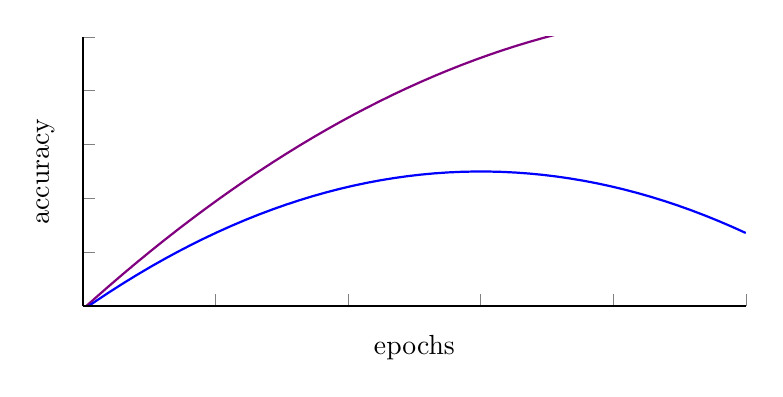
\begin{tikzpicture}
                        \begin{axis}[
                            axis on top=true,
                            axis line style=thick,
                            no markers, domain=0:10, samples=50,
                            axis lines*=left, xlabel=epochs, ylabel=accuracy,
                            height=5cm, width=10cm,
                            enlargelimits=false,
                            xticklabels={,,},
                            yticklabels={,,},
                            xmin=0, xmax=10,
                            ymin=0, ymax=10
                        ]
                            \addplot[violet, thick] {-(\x - 10) * (\x - 10) / 9 + 11};
                            \addplot[blue, thick] {-(\x - 6) * (\x - 6) / 7 + 5};
                        \end{axis}
                    \end{tikzpicture}
                \end{center}
                Note that the model will continue to become more accurate on the \violet{training data}, but accuracy on the \blue{validation data} will likely get worse as it overfits.
                We want to validate on the validation data every epoch, storing the best model so far, and stop training when the performance hasn't improved for a number of epochs.
                \medskip

                Another approach is \textbf{regularisation}, where we add information or constraints to stop the model from overfitting.
                An example of this is to restrict the weights of the model.
                The forms of regularisation are as follows;
                \begin{itemize}
                    \itemsep0em
                    \item \textbf{L2 regularisation}
                        \smallskip

                        We add the squared weights to the loss function (our new loss function is now $J(\theta)$).
                        We therefore penalise large weights, and push them towards 0 - this encourages sharing between features since small weights aren't penalised as much.
                        $$J(\theta) = \text{Loss}(y, \hat{y}) + \lambda \summation{w}{} w^2 \Rightarrow w \leftarrow w - \alpha\left(\pdif{\text{Loss}}{w} + 2\lambda w\right)$$
                        Since the weights are in the update, it reduces the weight on every update.
                    \item \textbf{L1 regularisation}
                        \smallskip

                        Similar to the above, but using absolute weights - this encourages sparsity as the model only keeps the most important features (by encouraging unnecessary weights towards 0);
                        $$J(\theta) = \text{Loss}(y, \hat{y}) + \lambda \summation{w}{} | w | \Rightarrow w \leftarrow w - \alpha\left(\pdif{\text{Loss}}{w} + \lambda \cdot \text{sign}(w)\right)$$
                \end{itemize}
                Another approach is \textbf{dropout}.
                This sets some neural activations to 0, and typically we drop around half of the activations in a layer.
                This prevents the network from relying on any one node.
        \subsection*{Week 7 (Unsupervised Learning)}
        \subsection*{Week 8 (Genetic Algorithms)}
\end{document}